
% !TeX program = xelatex
\documentclass[11pt,a4paper]{article}

% -------------------------------------------------
% Packages
% -------------------------------------------------
\usepackage{kotex}
\usepackage{fontspec}
\usepackage{amsmath,amssymb,bm,mathtools}
\usepackage[left=24mm,right=24mm,top=23mm,bottom=25mm]{geometry}
\usepackage{booktabs,array}
\usepackage{enumitem}
\usepackage{setspace}
\usepackage{xcolor}
\usepackage{colortbl}
\usepackage{tikz}
\usetikzlibrary{positioning,arrows.meta,calc,fit}
\usepackage[most]{tcolorbox}
\usepackage{listings}
\usepackage{hyperref}
\usepackage{fancyhdr}

\setstretch{1.14}
\setlength{\parindent}{0pt}
\setlength{\parskip}{0.55em}

% -------------------------------------------------
% Colors and boxes
% -------------------------------------------------
\definecolor{deepblue}{RGB}{34,71,120}
\definecolor{softblue}{RGB}{239,246,253}
\definecolor{softgray}{RGB}{246,247,249}
\definecolor{softgreen}{RGB}{239,249,242}
\definecolor{softyellow}{RGB}{255,249,229}
\definecolor{codegray}{RGB}{248,248,248}

\newtcolorbox{keybox}[1][]{
  colback=softblue,
  colframe=deepblue,
  boxrule=0.7pt,
  arc=2mm,
  title=#1,
  fonttitle=\bfseries
}

\newtcolorbox{thinkbox}[1][]{
  colback=softyellow,
  colframe=orange!70!black,
  boxrule=0.6pt,
  arc=2mm,
  title=#1,
  fonttitle=\bfseries
}

\newtcolorbox{remarkbox}[1][]{
  colback=softgray,
  colframe=black!45,
  boxrule=0.5pt,
  arc=2mm,
  title=#1,
  fonttitle=\bfseries
}

\newtcolorbox{mlbox}[1][]{
  colback=softgreen,
  colframe=green!45!black,
  boxrule=0.6pt,
  arc=2mm,
  title=#1,
  fonttitle=\bfseries
}

% -------------------------------------------------
% Code style
% -------------------------------------------------
\lstdefinestyle{pythonstyle}{
  language=Python,
  backgroundcolor=\color{codegray},
  basicstyle=\ttfamily\small,
  keywordstyle=\bfseries,
  commentstyle=\itshape\color{black!60},
  stringstyle=\color{black!75},
  numbers=left,
  numberstyle=\tiny\color{black!55},
  numbersep=8pt,
  frame=single,
  rulecolor=\color{black!25},
  breaklines=true,
  showstringspaces=false,
  tabsize=4,
  columns=fullflexible,
  keepspaces=true
}
\lstset{style=pythonstyle}

% -------------------------------------------------
% Math commands
% -------------------------------------------------
\newcommand{\R}{\mathbb{R}}
\newcommand{\grad}{\nabla}
\newcommand{\vect}[1]{\bm{#1}}
\newcommand{\T}{^{\mathsf T}}
\newcommand{\loss}{\mathcal{L}}
\newcommand{\sigmoid}{\sigma}

% -------------------------------------------------
% Header / footer
% -------------------------------------------------
\pagestyle{fancy}
\fancyhf{}
\lhead{Introduction to Deep Learning and Practice}
\rhead{Neuron, Activation, and Hidden Layer}
\cfoot{\thepage}
\renewcommand{\headrulewidth}{0.4pt}
\setlength{\headheight}{14pt}

\hypersetup{
  colorlinks=true,
  linkcolor=deepblue,
  urlcolor=deepblue
}

% =================================================
\begin{document}
% =================================================

\begin{center}
{\LARGE\bfseries Neuron에서 Hidden Layer까지}\\[0.35em]
{\Large Perceptron $\rightarrow$ Activation $\rightarrow$ Classification
$\rightarrow$ Universal Approximation}\\[0.8em]
\end{center}

\vspace{0.4em}

\begin{keybox}[이번 주의 핵심 질문]
하나의 affine function
\[
a=\vect{w}\T\vect{x}+b
\]
만으로는 표현할 수 있는 함수의 형태가 매우 제한적이다.
그렇다면 neural network는 어떻게 비선형적인 함수와 복잡한 분류 문제를 표현할 수 있을까?

하나의 neuron을 수식과 computational graph로 나타내고,
activation function이 왜 필요한지 이해한다.
그 다음 하나의 sigmoid neuron을 이용한 binary classification을 직접 학습하고,
마지막으로 여러 neuron을 hidden layer에 배치하면 왜 훨씬 복잡한 함수를 표현할 수 있는지 살펴본다.
\end{keybox}

\subsection*{학습목표}

이 주차가 끝나면 다음을 설명하고 직접 계산할 수 있어야 한다.

\begin{enumerate}[label=\arabic*.]

\item activation function의 역할과 비선형성이 필요한 이유를 설명한다.
\item sigmoid, tanh, ReLU의 기본 형태와 local derivative를 사용할 수 있다.
\item 하나의 sigmoid neuron을 computational graph로 나타내고 backward derivative를 계산한다.
\item 1차원 binary classification에서 decision boundary의 의미를 설명한다.
\item single neuron이 표현할 수 없는 패턴을 설명하고 hidden layer의 필요성을 이해한다.
\item one-hidden-layer network가 비선형 함수를 근사하는 구조를 설명한다.
\item Universal Approximation Theorem의 의미와 한계를 설명한다.
\end{enumerate}


% =================================================
% =================================================

\subsection*{Artificial Intelligence, Machine Learning, Deep Learning}

인공지능(Artificial Intelligence, AI)은 인간이 수행하는 인식, 판단, 예측,
문제 해결과 같은 지적인 작업을 컴퓨터가 수행하도록 만드는 연구 분야를 넓게 가리킨다.
인공지능을 구현하는 방법에는 여러 가지가 있으며, 그중 하나가
machine learning이다.

Machine learning은 사람이 모든 규칙을 직접 프로그램하는 대신,
데이터로부터 모델의 규칙이나 parameter를 학습하도록 하는 방법이다.
즉, 데이터
\[
(x_i,t_i),\qquad i=1,\ldots,N
\]
가 주어졌을 때, 어떤 모델
\[
f(x;\theta)
\]
의 parameter $\theta$를 데이터로부터 결정하는 것이 machine learning의
가장 기본적인 형태라고 볼 수 있다.

Artificial neural network(ANN)는 machine learning에 사용되는 모델의 한 종류이다.
여러 개의 artificial neuron을 서로 연결하여 하나의 복잡한 함수를 구성한다.

그중에서도 여러 개의 layer를 갖는 neural network를 이용하여
데이터로부터 복잡한 representation을 학습하는 방법을
deep learning이라고 한다.

따라서 개념적인 포함관계는

\[
\boxed{
\text{Artificial Intelligence}
\supset
\text{Machine Learning}
\supset
\text{Artificial Neural Networks}
\supset
\text{Deep Learning}
}
\]

으로 생각할 수 있다.

여기서 한 가지 주의할 점은 artificial neural network와 deep learning이
완전히 같은 의미는 아니라는 것이다.
하나 또는 소수의 layer만을 갖는 neural network도 존재하며,
deep learning은 일반적으로 여러 layer를 갖는 neural network를 이용하여
복잡한 함수를 학습하는 방법을 의미한다.

\subsection*{Artificial Neural Network는 어디에서 시작되었는가?}

오늘날 인공지능 연구의 중요한 발전을 이끌고 있는 deep learning의 뿌리는
오래전부터 연구되어 온 artificial neural network(ANN)에 있다.
Artificial neural network는 생물학적인 신경망에서 영감을 받아 만들어진
computational model이다.

``스스로 학습하고 판단하는 기계''를 만드는 것은 오랫동안 인간의 꿈이었다.
초기의 인공지능 연구자들은 인간의 뇌가 정보를 처리하는 방식에서 아이디어를 얻어,
뇌의 기본 단위인 신경세포, 즉 neuron에 관심을 가졌다.

생물학적인 neuron은 다른 neuron으로부터 여러 신호를 받아들이고,
이 신호들을 종합한 뒤 일정한 조건이 만족되면 다시 다른 neuron으로
신호를 전달한다.
중요한 점은 인간의 뇌가 하나의 neuron만으로 복잡한 판단을 수행하는 것이 아니라,
매우 많은 neuron이 서로 연결된 network를 이용한다는 것이다.

이러한 아이디어로부터 다음과 같은 단순한 computational unit을 생각할 수 있다.

\[
a=w_1x_1+w_2x_2+\cdots+w_nx_n+b,
\]

그리고 이 weighted sum에 어떤 함수 $\phi$를 적용하여

\[
z=\phi(a)
\]

를 출력하도록 한다.

즉,

\[
\boxed{
z=
\phi\!\left(
w_1x_1+\cdots+w_nx_n+b
\right)
}
\]

와 같은 매우 단순한 계산을 하나의 artificial neuron이 수행한다고 생각한다.

여기서 $x_1,\ldots,x_n$은 다른 neuron 또는 외부로부터 들어오는 입력신호이고,
$w_1,\ldots,w_n$은 각 입력신호의 중요도를 나타내는 weight,
$b$는 bias이다.
함수 $\phi$는 입력신호의 weighted sum을 실제 출력신호로 변환하며
activation function이라고 부른다.

Artificial neural network는 이러한 단순한 unit 또는 node를
많이 연결하여 만든다.
각 node의 출력은 다시 다른 node의 입력이 되고,
이러한 계산이 여러 layer를 따라 반복된다.

\[
\text{input}
\longrightarrow
\text{simple computations}
\longrightarrow
\text{simple computations}
\longrightarrow
\cdots
\longrightarrow
\text{output}.
\]

하나의 neuron이 할 수 있는 계산은 매우 단순하다.
그러나 많은 neuron을 서로 연결하고 그 사이에 nonlinear activation을 넣으면
전체 network는 매우 복잡한 함수를 표현할 수 있다.

바로 이 점이 neural network의 핵심 아이디어이다.

\begin{keybox}[Neural network를 하나의 거대한 함수로 보기]
Neural network를 생물학적인 뇌의 모형으로만 생각할 필요는 없다.
수학적으로는 많은 간단한 함수들을 반복적으로 합성하여 만들어진
하나의 매우 복잡한 함수라고 생각할 수 있다.

\[
\boxed{
\text{Neural Network}
=
\text{Composition of many simple functions}
}
\]

그리고 learning이란 이 함수 안에 들어 있는 수많은 weight와 bias를
데이터로부터 결정하는 과정이다.
\end{keybox}


\section{Artificial Neuron과 Perceptron}
% =================================================



\subsection{하나의 neuron은 무엇을 계산하는가?}

입력 vector를
\[
\vect{x}
=
\begin{bmatrix}
x_1\\
x_2\\
\vdots\\
x_n
\end{bmatrix},
\qquad
\vect{w}
=
\begin{bmatrix}
w_1\\
w_2\\
\vdots\\
w_n
\end{bmatrix}
\]
라고 하자.

하나의 artificial neuron은 먼저 입력의 가중합(weighted sum)
\[
\boxed{
a=\vect{w}\T\vect{x}+b
=
\sum_{j=1}^{n}w_jx_j+b
}
\]
을 계산하고, 그 결과에 activation function $\phi$를 적용하여
\[
\boxed{
z=\phi(a)
}
\]
를 출력한다.

따라서 하나의 neuron은
\[
\boxed{
\vect{x}
\longrightarrow
a=\vect{w}\T\vect{x}+b
\longrightarrow
z=\phi(a)
}
\]
라는 두 단계의 합성함수로 볼 수 있다.

\begin{center}
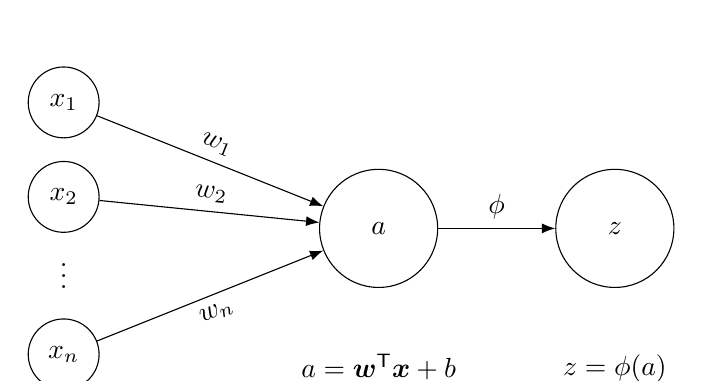
\begin{tikzpicture}[>=Latex]
\node[draw,circle,minimum size=9mm] (x1) at (0,1.8) {$x_1$};
\node[draw,circle,minimum size=9mm] (x2) at (0,0.6) {$x_2$};
\node[draw=none] (vd) at (0,-0.3) {$\vdots$};
\node[draw,circle,minimum size=9mm] (xn) at (0,-1.4) {$x_n$};

\node[draw,circle,minimum size=15mm] (a) at (4,0.2) {$a$};
\node[draw,circle,minimum size=15mm] (z) at (7,0.2) {$z$};

\draw[->] (x1) -- node[above,sloped] {$w_1$} (a);
\draw[->] (x2) -- node[above,sloped] {$w_2$} (a);
\draw[->] (xn) -- node[below,sloped] {$w_n$} (a);
\draw[->] (a) -- node[above] {$\phi$} (z);

\node[draw=none,below=0.72cm of a] {$a=\vect{w}\T\vect{x}+b$};
\node[draw=none,below=0.72cm of z] {$z=\phi(a)$};
\end{tikzpicture}
\end{center}

여기서 $w_j$는 각 입력 $x_j$가 neuron에 미치는 영향의 크기를 정하고,
$b$는 전체 weighted sum을 이동시키는 역할을 한다.

\subsection{Classical perceptron}

고전적인 perceptron에서는 activation function으로 step function을 사용한다.

\[
H(a)
=
\begin{cases}
0, & a\le 0,\\
1, & a>0.
\end{cases}
\]

따라서 perceptron의 출력은
\[
\boxed{
z
=
H\!\left(\vect{w}\T\vect{x}+b\right)
}
\]
이다.

즉,
\[
\vect{w}\T\vect{x}+b>0
\]
이면 $1$을 출력하고 그렇지 않으면 $0$을 출력한다.

\begin{remarkbox}[Perceptron과 modern artificial neuron]
고전적인 의미의 perceptron은 step activation을 사용하는 threshold classifier를 가리킨다.
현대의 neural network에서는 같은 weighted-sum 구조를 유지하면서
step function 대신 sigmoid, tanh, ReLU와 같은 activation function을 사용한다.
이 강의에서는 필요에 따라 ``neuron''이라는 더 일반적인 표현을 사용한다.
\end{remarkbox}

\subsection{1차원에서는 무엇을 하는가?}

입력이 하나라면
\[
a=wx+b
\]
이고 perceptron은
\[
z=H(wx+b)
\]
이다.

$w\neq0$일 때 출력이 바뀌는 위치는
\[
wx+b=0
\]
이므로
\[
\boxed{
x=-\frac{b}{w}
}
\]
이다.

즉 1차원 perceptron은 실수축을 하나의 경계점으로 나누어 두 class로 분류한다.

% =================================================
\section{Activation Function}
% =================================================

\subsection{왜 step function만으로는 학습하기 어려운가?}

step function은 $a=0$에서 미분가능하지 않고, $a\neq0$에서는
\[
H'(a)=0
\]
이다.

gradient descent로 parameter를 학습하려면
\[
\frac{\partial L}{\partial w},
\qquad
\frac{\partial L}{\partial b}
\]
와 같은 derivative가 필요하다.
그러나 activation의 derivative가 거의 모든 곳에서 $0$이면
gradient가 앞쪽 parameter로 전달되지 않는다.

따라서 gradient-based learning을 위해서는
\textbf{미분가능하거나 거의 모든 곳에서 유용한 derivative를 갖는 activation function}이 필요하다.

\subsection{Sigmoid function}

가장 대표적인 smooth activation 중 하나는 logistic sigmoid이다.

\[
\boxed{
\sigmoid(a)
=
\frac{1}{1+e^{-a}}
}
\]

sigmoid는 모든 실수 입력을 $(0,1)$ 사이의 값으로 보낸다.

특히 derivative는
\[
\boxed{
\sigmoid'(a)
=
\sigmoid(a)\bigl(1-\sigmoid(a)\bigr)
}
\]
이다.

따라서 forward에서
\[
z=\sigmoid(a)
\]
를 이미 계산해 두었다면 backward에서는
\[
\boxed{
\frac{dz}{da}=z(1-z)
}
\]
로 바로 사용할 수 있다.

\begin{thinkbox}[Forward에서 계산한 값을 backward에서 다시 사용한다]
앞 주차에서 보았듯 backpropagation은 graph를 거꾸로 따라가며 local derivative를 곱한다.
sigmoid에서는 forward에서 계산한 $z$ 자체가
\[
\frac{dz}{da}=z(1-z)
\]
를 계산하는 데 사용된다.
실제 neural network framework에서도 forward 과정의 중간값을 저장해 두었다가 backward에서 재사용하는 구조가 중요하다.
\end{thinkbox}

\subsection{Tanh와 ReLU}

자주 사용되는 activation을 몇 가지 정리하면 다음과 같다.

\[
\tanh(a)
=
\frac{e^a-e^{-a}}{e^a+e^{-a}},
\qquad
\boxed{
\frac{d}{da}\tanh(a)=1-\tanh^2(a)
}
\]

그리고 ReLU(Rectified Linear Unit)는
\[
\boxed{
\operatorname{ReLU}(a)=\max(0,a)
}
\]
이고 $a\neq0$에서
\[
\operatorname{ReLU}'(a)
=
\begin{cases}
0,&a<0,\\
1,&a>0.
\end{cases}
\]

\begin{center}
\begin{tabular}{c|c|c|c}
\toprule
Activation & Output range & Derivative & 특징\\
\midrule
Step & $\{0,1\}$ & $0$ a.e. & classical perceptron\\
Sigmoid & $(0,1)$ & $z(1-z)$ & binary output에 직관적\\
Tanh & $(-1,1)$ & $1-z^2$ & zero-centered output\\
ReLU & $[0,\infty)$ & $0$ or $1$ & modern hidden layer에 널리 사용\\
\bottomrule
\end{tabular}
\end{center}

이 주차에서는 sigmoid를 중심으로 계산하고,
tanh와 ReLU는 이후 network 구조를 다룰 때 다시 사용한다.

% =================================================
\section{왜 Nonlinearity가 필요한가?}
% =================================================

activation function의 가장 중요한 수학적 역할은
단순히 생물학적 neuron의 ``활성/비활성''을 흉내 내는 것에 있지 않다.
핵심은 network에 \textbf{nonlinearity}를 넣는 것이다.

두 affine transformation을 생각하자.

\[
\vect{u}=W_1\vect{x}+\vect{b}_1,
\qquad
\vect{y}=W_2\vect{u}+\vect{b}_2.
\]

이를 합성하면
\[
\begin{aligned}
\vect{y}
&=
W_2(W_1\vect{x}+\vect{b}_1)+\vect{b}_2\\
&=
(W_2W_1)\vect{x}+(W_2\vect{b}_1+\vect{b}_2).
\end{aligned}
\]

즉,
\[
\boxed{
\text{affine}\circ\text{affine}
=
\text{affine}
}
\]
이다.

affine layer를 2개, 20개, 200개 쌓더라도
중간에 nonlinear activation이 없다면 전체 mapping은 결국 하나의 affine mapping과 같다.

\begin{keybox}[Activation function의 수학적 역할]
Neural network가 복잡한 함수를 표현하려면
\[
\boxed{
\text{Affine transformation}
\quad+\quad
\text{Nonlinear activation}
}
\]
의 반복이 필요하다.

Network의 ``깊이''만 늘리는 것으로는 충분하지 않다.
비선형성이 들어가야 표현력이 증가한다.
\end{keybox}

% =================================================
\section{하나의 Sigmoid Neuron으로 Binary Classification}
% =================================================

\subsection{Binary classification}

다음 데이터를 생각하자.

\[
\begin{array}{c|ccccc}
x_i & -2 & -1 & 0 & 1 & 2\\
\hline
t_i & 0 & 0 & 1 & 1 & 1
\end{array}
\]

%\includegraphics[width=0.5\textwidth]{./figures/binary_classification.png}

target $t_i$가 $0$ 또는 $1$의 두 값만 가지므로 binary classification 문제이다.

하나의 sigmoid neuron을 사용하여
\[
\boxed{
a_i=wx_i+b,
\qquad
z_i=\sigmoid(a_i)
}
\]
를 예측모델로 사용하자.

$z_i$는 $(0,1)$ 사이의 연속적인 값을 출력한다.
이를 class label로 바꾸기 위해 예를 들어
\[
\widehat t_i
=
\begin{cases}
1,&z_i\ge 0.5,\\
0,&z_i<0.5
\end{cases}
\]
로 정할 수 있다.

sigmoid는
\[
\sigmoid(0)=0.5
\]
이고 증가함수이므로
\[
z_i\ge0.5
\quad\Longleftrightarrow\quad
wx_i+b\ge0.
\]

따라서 decision boundary는
\[
\boxed{
x=-\frac{b}{w}
}
\qquad(w\neq0)
\]
이다.

\subsection{Computational graph}

한 개의 datum $(x,t)$에 대해 다음 변수를 정의하자.

\[
a=wx+b,
\qquad
z=\sigmoid(a),
\qquad
e=z-t,
\qquad
\ell=e^2.
\]

그러면 computational graph는

\[
(x,w,b)
\longrightarrow
a
\longrightarrow
z
\longrightarrow
e
\longrightarrow
\ell
\]

이다.

\begin{center}
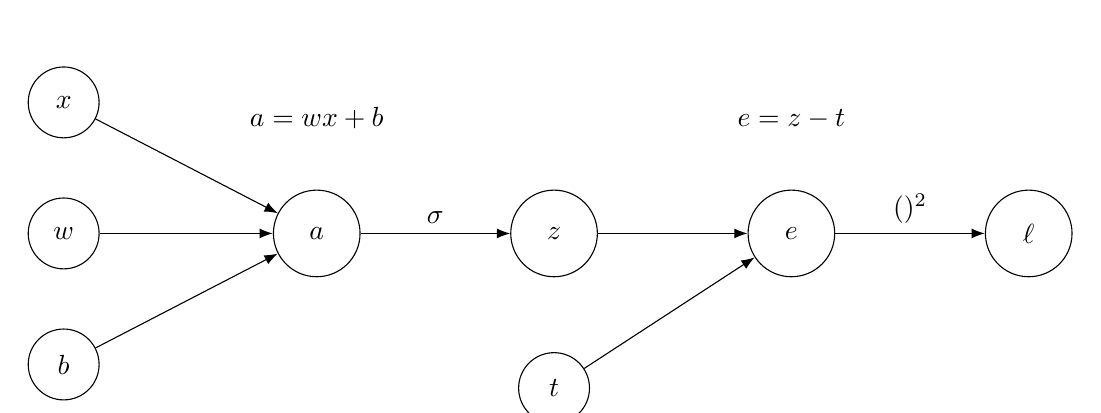
\begin{tikzpicture}[>=Latex,node distance=1.7cm]
\node[draw,circle,minimum size=9mm] (x) {$x$};
\node[draw,circle,minimum size=9mm,below=0.75cm of x] (w) {$w$};
\node[draw,circle,minimum size=9mm,below=0.75cm of w] (b) {$b$};

\node[draw,circle,minimum size=11mm,right=2.2cm of w] (a) {$a$};
\node[draw,circle,minimum size=11mm,right=1.9cm of a] (z) {$z$};
\node[draw,circle,minimum size=9mm,below=0.95cm of z] (t) {$t$};
\node[draw,circle,minimum size=11mm,right=1.9cm of z] (e) {$e$};
\node[draw,circle,minimum size=11mm,right=1.9cm of e] (l) {$\ell$};

\draw[->] (x) -- (a);
\draw[->] (w) -- (a);
\draw[->] (b) -- (a);
\draw[->] (a) -- node[above] {$\sigmoid$} (z);
\draw[->] (z) -- (e);
\draw[->] (t) -- (e);
\draw[->] (e) -- node[above] {$()^2$} (l);

\node[draw=none,above=0.65cm of a] {$a=wx+b$};
\node[draw=none,above=0.65cm of e] {$e=z-t$};
\end{tikzpicture}
\end{center}

\subsection{Backward: local derivative를 따라가기}

각 edge에서 필요한 local derivative는

\[
\frac{\partial\ell}{\partial e}=2e,
\qquad
\frac{\partial e}{\partial z}=1,
\qquad
\frac{\partial z}{\partial a}=z(1-z),
\]
\[
\frac{\partial a}{\partial w}=x,
\qquad
\frac{\partial a}{\partial b}=1.
\]

따라서 chain rule에 의해

\[
\boxed{
\frac{\partial\ell}{\partial w}
=
\frac{\partial\ell}{\partial e}
\frac{\partial e}{\partial z}
\frac{\partial z}{\partial a}
\frac{\partial a}{\partial w}
=
2e\,z(1-z)x
}
\]

이고

\[
\boxed{
\frac{\partial\ell}{\partial b}
=
2e\,z(1-z)
}
\]
이다.

즉 linear output 뒤에 sigmoid node 하나가 추가되면서
backward에서도 local derivative
\[
z(1-z)
\]
하나가 추가된 것이다.

\begin{mlbox}[Backpropagation의 관점]
Forward:
\[
x,w,b
\longrightarrow a
\longrightarrow z
\longrightarrow e
\longrightarrow \ell.
\]

Backward:
\[
\frac{\partial\ell}{\partial e}
\longrightarrow
\frac{\partial\ell}{\partial z}
\longrightarrow
\frac{\partial\ell}{\partial a}
\longrightarrow
\left(
\frac{\partial\ell}{\partial w},
\frac{\partial\ell}{\partial b}
\right).
\]

Network가 길어져도 원리는 같다.
뒤쪽에서 전달된 gradient에 현재 node의 local derivative를 곱하여 앞쪽으로 전달한다.
\end{mlbox}

\subsection{여러 데이터에 대한 gradient}

$N$개의 데이터 $(x_i,t_i)$에 대해 이 주차에서는 계산 구조를 명확하게 보기 위해
MSE loss를 사용하자.

\[
L(w,b)
=
\frac1N\sum_{i=1}^{N}(z_i-t_i)^2,
\qquad
z_i=\sigmoid(wx_i+b).
\]

그러면

\[
\boxed{
\frac{\partial L}{\partial w}
=
\frac{2}{N}
\sum_{i=1}^{N}
(z_i-t_i)z_i(1-z_i)x_i
}
\]

\[
\boxed{
\frac{\partial L}{\partial b}
=
\frac{2}{N}
\sum_{i=1}^{N}
(z_i-t_i)z_i(1-z_i)
}
\]

이고 gradient descent는

\[
\begin{bmatrix}
w\\ b
\end{bmatrix}
\leftarrow
\begin{bmatrix}
w\\ b
\end{bmatrix}
-
\eta
\begin{bmatrix}
\partial L/\partial w\\
\partial L/\partial b
\end{bmatrix}
\]
로 수행한다.

\begin{remarkbox}[Classification loss에 대한 참고]
Binary classification에서는 binary cross-entropy(BCE)가 더 표준적인 loss이다.
하지만 이번 주에는 activation node가 추가되었을 때 chain rule과 backward가 어떻게 바뀌는지를
선명하게 보기 위해 MSE를 사용한다.
BCE와 softmax/cross-entropy는 뒤에서 별도로 다룬다.
\end{remarkbox}

% =================================================
\section{Single Neuron의 한계}
% =================================================

하나의 sigmoid neuron은 1차원에서
\[
z(x)=\sigmoid(wx+b)
\]
형태이다.

$w>0$이면 증가함수이고,
$w<0$이면 감소함수이다.
따라서 하나의 sigmoid neuron은 본질적으로 하나의 transition만 만들 수 있다.

예를 들어 target이

\[
\begin{array}{c|ccccc}
x & -2 & -1 & 0 & 1 & 2\\
\hline
t & 0 & 1 & 1 & 1 & 0
\end{array}
\]

처럼 ``가운데만 class 1''이라면 하나의 threshold로는 분류할 수 없다.
class $0\to1$로 바뀌는 경계와 $1\to0$으로 바뀌는 경계가 두 개 필요하기 때문이다.

마찬가지로 하나의 sigmoid
\[
\sigmoid(wx+b)
\]
만으로는 $x^2$, $\sin x$와 같은 일반적인 non-monotone function을 근사하기 어렵다.

\begin{thinkbox}[무엇이 더 필요한가?]
하나의 neuron이 만드는 단순한 비선형 함수를 여러 개 만들어서
이들을 다시 조합하면 어떨까?

이 생각이 바로 \textbf{hidden layer}의 출발점이다.
\end{thinkbox}

% =================================================
\section{Hidden Layer와 Nonlinear Function Approximation}
% =================================================

\subsection{하나의 hidden layer}

입력 $x\in\R$에서 $m$개의 hidden neurons를 만드는 network를 생각하자.

각 hidden neuron에서
\[
a_j=x\,w_j^{(1)}+b_j^{(1)},
\qquad
h_j=\phi(a_j),
\qquad
j=1,\ldots,m
\]
를 계산하고, 마지막 출력에서는 이 hidden outputs를 다시 선형결합하여

\[
\boxed{
\widehat y
=
\sum_{j=1}^{m}
h_j\,w_j^{(2)}+b^{(2)}
}
\]
를 계산한다.

즉,

\[
\boxed{
\widehat y(x)
=
\sum_{j=1}^{m}
\phi\!\left(x\,w_j^{(1)}+b_j^{(1)}\right)
w_j^{(2)}
+b^{(2)}
}
\]

이다.

\begin{center}
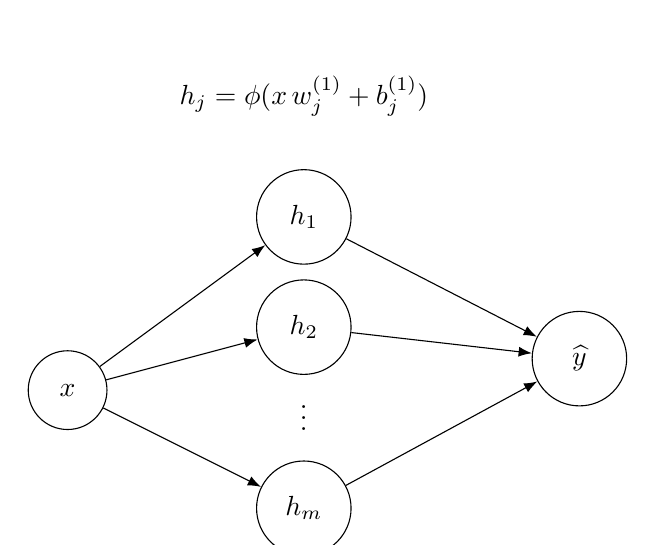
\begin{tikzpicture}[>=Latex]
\node[draw,circle,minimum size=10mm] (x) at (0,0) {$x$};

\node[draw,circle,minimum size=12mm] (h1) at (3,2.2) {$h_1$};
\node[draw,circle,minimum size=12mm] (h2) at (3,0.8) {$h_2$};
\node[draw=none] (vd) at (3,-0.25) {$\vdots$};
\node[draw,circle,minimum size=12mm] (hm) at (3,-1.5) {$h_m$};

\node[draw,circle,minimum size=12mm] (y) at (6.5,0.4) {$\widehat y$};

\draw[->] (x) -- (h1);
\draw[->] (x) -- (h2);
\draw[->] (x) -- (hm);
\draw[->] (h1) -- (y);
\draw[->] (h2) -- (y);
\draw[->] (hm) -- (y);

\node[draw=none,above=0.55cm of h1] {$h_j=\phi(x\,w_j^{(1)}+b_j^{(1)})$};
\end{tikzpicture}
\end{center}

입력과 출력 사이에 직접 관측되지 않는 중간 variables
\[
h_1,\ldots,h_m
\]
가 존재하므로 이 층을 \textbf{hidden layer}라고 부른다.

\subsection{Matrix form}

입력 $x$를 앞에, weight matrix를 뒤에 곱하는 \textbf{행벡터(row-vector) 규약}을 사용하자.
(NumPy, PyTorch 코드의 \texttt{X @ W + b}와 같은 순서이다.)

\[
W^{(1)}
=
\begin{bmatrix}
w_1^{(1)} & \cdots & w_m^{(1)}
\end{bmatrix}
\in\R^{1\times m},
\qquad
\vect{b}^{(1)}
=
\begin{bmatrix}
b_1^{(1)} & \cdots & b_m^{(1)}
\end{bmatrix}
\in\R^{1\times m}
\]
라고 두면

\[
\vect{a}
=
x\,W^{(1)}+\vect{b}^{(1)}
\in\R^{1\times m},
\qquad
\vect{h}
=
\phi(\vect{a})
\in\R^{1\times m}
\]
이고 ($\phi$는 성분별로 적용),

\[
\widehat y
=
\vect{h}\,\vect{w}^{(2)}+b^{(2)},
\qquad
\vect{w}^{(2)}
=
\begin{bmatrix}
w_1^{(2)}\\
\vdots\\
w_m^{(2)}
\end{bmatrix}
\in\R^{m\times1}
\]
로 compact하게 쓸 수 있다.

따라서 전체 network는

\[
\boxed{
x
\longrightarrow
\vect{a}
\longrightarrow
\vect{h}
\longrightarrow
\widehat y
}
\]

라는 합성함수이다.

\subsection{Hidden neuron은 서로 다른 nonlinear basis를 만든다}

sigmoid activation을 사용하면 각 hidden neuron은

\[
h_j(x)
=
\sigmoid\!\left(w_j^{(1)}x+b_j^{(1)}\right)
\]
와 같은 S-shaped function을 만든다.

$w_j^{(1)}$와 $b_j^{(1)}$가 달라지면
각 sigmoid의 기울기와 transition 위치가 달라진다.

마지막 output layer는 이 함수들을

\[
w_1^{(2)}h_1(x)
+\cdots+
w_m^{(2)}h_m(x)
+b^{(2)}
\]
와 같이 선형결합한다.

즉 hidden layer의 neuron들은 서로 다른 nonlinear ``building blocks''를 만들고,
output layer가 이들을 조합하여 더 복잡한 함수를 만든다.

% =================================================
\section{Universal Approximation의 직관}
% =================================================

\subsection{Sigmoid 두 개로 구간을 만들기}

먼저 sigmoid 하나를 평행이동하고 가로 방향으로 압축한 함수
\[
\sigmoid(k(x-a)),
\qquad k>0
\]
를 살펴보자.
hidden neuron $\sigmoid(x\,w+b)$에서 $w>0$이면
\[
x\,w+b=w\left(x-\left(-\tfrac{b}{w}\right)\right)
\]
이므로, $k=w$, $a=-b/w$인 경우에 해당한다.

\begin{center}
\begin{tikzpicture}[>=Latex,x=1.4cm,y=3.6cm]
% axes
\draw[->] (-3,0) -- (3.3,0) node[right] {$x$};
\draw[->] (-3,-0.05) -- (-3,1.15);
\draw[gray!60,dashed] (-3,1) -- (3,1);
\node[left] at (-3,1) {$1$};
\node[left] at (-3,0.5) {$\tfrac12$};
\node[left] at (-3.03,0) {$0$};
\draw (-3.05,0.5) -- (-2.95,0.5);
\draw[gray!60,dashed] (0,0) -- (0,1.05);
\node[below] at (0,0) {$a$};

% sigma(k(x-a)), plotted in t = x-a
\draw[thick,blue!70!black,domain=-3:3,samples=80]
  plot (\x,{1/(1+exp(-1*\x))});
\draw[thick,orange!85!black,domain=-3:3,samples=100]
  plot (\x,{1/(1+exp(-3*\x))});
\draw[thick,red!75!black]
  (-3,0) -- plot[domain=-0.9:0.9,samples=120] (\x,{1/(1+exp(-10*\x))}) -- (3,1);

% tangent lines at x=a: y = 1/2 + (k/4)(x-a)
\draw[dashed,blue!70!black] (-2,0) -- (2,1);
\draw[dashed,orange!85!black] (-2/3,0) -- (2/3,1);
\draw[dashed,red!75!black] (-0.2,0) -- (0.2,1);

\fill (0,0.5) circle (1.4pt);

% legend
\begin{scope}[shift={(-2.85,0.62)}]
\draw[thick,blue!70!black] (0,0.28) -- (0.4,0.28);
\draw[thick,orange!85!black] (0,0.14) -- (0.4,0.14);
\draw[thick,red!75!black] (0,0) -- (0.4,0);
\node[right] at (0.4,0.28) {\small $k=1$:\ 기울기 $1/4$};
\node[right] at (0.4,0.14) {\small $k=3$:\ 기울기 $3/4$};
\node[right] at (0.4,0) {\small $k=10$:\ 기울기 $10/4$};
\end{scope}
\end{tikzpicture}

\small 실선: $\sigmoid(k(x-a))$,\quad 점선: $x=a$에서의 접선
\end{center}

모든 $k$에 대하여 $\sigmoid(k(x-a))$는 점 $\left(a,\tfrac12\right)$를 지난다.
즉 $a$는 함수가 $0$ 쪽에서 $1$ 쪽으로 넘어가는 \textbf{위치}를 정하고,
$k$는 그 변화가 얼마나 \textbf{가파른지}를 정한다.

이를 미분으로 확인하자.
$z=k(x-a)$라 두면 $\dfrac{dz}{dx}=k$이고,
sigmoid의 derivative $\sigmoid'(z)=\sigmoid(z)\bigl(1-\sigmoid(z)\bigr)$와 chain rule에 의해
\[
\frac{d}{dx}\sigmoid(k(x-a))
=
\sigmoid'(z)\,\frac{dz}{dx}
=
k\,\sigmoid(k(x-a))\bigl(1-\sigmoid(k(x-a))\bigr)
\]
이다.
$x=a$에서는 $z=0$이고 $\sigmoid(0)=\tfrac12$이므로
\[
\boxed{
\left.\frac{d}{dx}\sigmoid(k(x-a))\right|_{x=a}
=
k\cdot\frac12\cdot\left(1-\frac12\right)
=
\frac{k}{4}
}
\]
를 얻는다.

따라서 $x=a$에서의 접선은
\[
y=\frac12+\frac{k}{4}(x-a)
\]
이고, 이 접선은 $x=a-\tfrac{2}{k}$에서 $y=0$, $x=a+\tfrac{2}{k}$에서 $y=1$이 된다.
즉 함수가 $0$ 근처에서 $1$ 근처로 바뀌는 구간의 폭은 대략 $\tfrac{4}{k}$이다.

\begin{keybox}[$k$가 커지면 sigmoid는 step function에 가까워진다]
$x=a$에서의 기울기 $\tfrac{k}{4}$는 $k$에 비례하여 커지고,
전이 구간의 폭 $\tfrac{4}{k}$는 $0$으로 줄어든다.
실제로 $k\to\infty$이면
\[
\sigmoid(k(x-a))
\longrightarrow
\begin{cases}
0,& x<a,\\[2pt]
\tfrac12,& x=a,\\[2pt]
1,& x>a
\end{cases}
\]
이므로, 큰 $k$에 대한 sigmoid는 $x=a$에서 뛰어오르는 step function처럼 행동한다.
\end{keybox}

정리하면, 큰 양수 $k$에 대하여
\[
\sigmoid(k(x-a))
\]
는 $x=a$ 근처에서 $0$에서 $1$로 빠르게 변한다.

따라서 두 sigmoid의 차

\[
\boxed{
r_{a,b}(x)
=
\sigmoid(k(x-a))
-
\sigmoid(k(x-b))
}
\qquad (a<b)
\]
는 $k$가 충분히 클 때 대략

\[
r_{a,b}(x)
\approx
\begin{cases}
1,&a<x<b,\\
0,&\text{otherwise}
\end{cases}
\]
와 같은 rectangular bump를 만든다.

\begin{center}
\begin{tikzpicture}[>=Latex,x=0.9cm,y=2.6cm,
  declare function={sig(\z)=1/(1+exp(-max(-9,min(9,\z))));}]
% ---------- (i) two sigmoids and their difference ----------
\begin{scope}
\draw[->] (-3,0) -- (3.3,0) node[right] {$x$};
\draw[->] (-3,-0.05) -- (-3,1.2);
\draw (-3.05,1) -- (-2.95,1);
\node[left] at (-3.03,1) {$1$};
\node[left] at (-3.03,0) {$0$};
\draw (-1,0.03) -- (-1,-0.03) node[below] {$a$};
\draw (1,0.03) -- (1,-0.03) node[below] {$b$};
\draw[very thick,red!75!black,domain=-3:3,samples=150]
  plot (\x,{sig(4*(\x+1))-sig(4*(\x-1))});
\draw[thick,dashed,blue!70!black,domain=-3:3,samples=100]
  plot (\x,{sig(4*(\x+1))});
\draw[thick,dashed,orange!85!black,domain=-3:3,samples=100]
  plot (\x,{sig(4*(\x-1))});
\node at (0,1.33) {\small (i) 두 sigmoid의 차 ($k=4$)};
% legend
\draw[thick,dashed,blue!70!black] (-2.6,-0.32) -- (-2,-0.32);
\node[right] at (-2,-0.32) {\small $\sigmoid(k(x-a))$};
\draw[thick,dashed,orange!85!black] (-2.6,-0.47) -- (-2,-0.47);
\node[right] at (-2,-0.47) {\small $\sigmoid(k(x-b))$};
\draw[very thick,red!75!black] (-2.6,-0.62) -- (-2,-0.62);
\node[right] at (-2,-0.62) {\small $r_{a,b}(x)=\sigmoid(k(x-a))-\sigmoid(k(x-b))$};
\end{scope}

% ---------- (ii) r_{a,b} vs. ideal rectangular bump ----------
\begin{scope}[xshift=7.8cm]
\fill[gray!18] (-1,0) rectangle (1,1);
\draw[->] (-3,0) -- (3.3,0) node[right] {$x$};
\draw[->] (-3,-0.05) -- (-3,1.2);
\draw (-3.05,1) -- (-2.95,1);
\node[left] at (-3.03,1) {$1$};
\node[left] at (-3.03,0) {$0$};
\draw (-1,0.03) -- (-1,-0.03) node[below] {$a$};
\draw (1,0.03) -- (1,-0.03) node[below] {$b$};
\draw[thick,gray!70] (-3,0) -- (-1,0) -- (-1,1) -- (1,1) -- (1,0) -- (3,0);
\draw[thick,blue!70!black,domain=-3:3,samples=100]
  plot (\x,{sig(2*(\x+1))-sig(2*(\x-1))});
\draw[thick,orange!85!black,domain=-3:3,samples=150]
  plot (\x,{sig(5*(\x+1))-sig(5*(\x-1))});
\draw[thick,red!75!black,domain=-3:3,samples=250]
  plot (\x,{sig(20*(\x+1))-sig(20*(\x-1))});
\node at (0,1.33) {\small (ii) $k$가 커질수록 rectangular bump에 가까워진다};
% legend
\fill[gray!18] (-2.6,-0.36) rectangle (-2,-0.28);
\draw[thick,gray!70] (-2.6,-0.32) -- (-2,-0.32);
\node[right] at (-2,-0.32) {\small rectangular bump $\mathbf 1_{(a,b)}(x)$};
\draw[thick,blue!70!black] (-2.6,-0.47) -- (-2,-0.47);
\node[right] at (-2,-0.47) {\small $r_{a,b}(x)$, $k=2$};
\draw[thick,orange!85!black] (-2.6,-0.62) -- (-2,-0.62);
\node[right] at (-2,-0.62) {\small $r_{a,b}(x)$, $k=5$};
\draw[thick,red!75!black] (-2.6,-0.77) -- (-2,-0.77);
\node[right] at (-2,-0.77) {\small $r_{a,b}(x)$, $k=20$};
\end{scope}
\end{tikzpicture}
\end{center}

즉 hidden neuron들의 선형결합만으로도
특정 구간에서만 값이 큰 함수를 만들 수 있다.

\subsection{Rectangular bumps를 더하면 일반적인 함수를 근사할 수 있다}

연속함수 $f$가 구간 $[a,b]$에 있다고 하자.
구간을 작은 조각들로 나누고 각 구간에서 $f$의 값을 하나의 상수로 근사하면
piecewise constant function을 얻는다.

각 piece는 앞의 rectangular bump로 근사할 수 있으므로

\[
f(x)
\approx
\sum_{j=1}^{m}
c_j
\left[
\sigmoid(k(x-a_j))
-
\sigmoid(k(x-a_{j+1}))
\right].
\]

예를 들어 $f(x)=x^2+2$를 $[0,4]$에서 같은 폭의 $m$개 구간
$[x_j,x_{j+1}]$ $(x_j=4j/m)$으로 나누고,
각 구간의 왼쪽 끝 값 $c_j=f(x_j)$를 높이로 사용하자.
$k=100$으로 고정하고 각 bump $c_j\,r_{x_j,x_{j+1}}(x)$를 더하면(superposition)
아래와 같이 $f$를 계단 모양으로 근사한다.
왼쪽($m=4$, $c=2,3,6,11$)은 3차시 실습 Step 7과 같은 구간 설정이다.

\begin{center}
\begin{tikzpicture}[>=Latex,x=1.4cm,y=0.17cm,
  declare function={
    sig(\z)=1/(1+exp(-max(-9,min(9,\z))));
    rb(\u,\p,\q)=sig(100*(\u-\p))-sig(100*(\u-\q));
  }]
% ---------- (i) m = 4 ----------
\begin{scope}
\draw[->] (-0.4,0) -- (4.6,0) node[right] {$x$};
\draw[->] (-0.4,-0.5) -- (-0.4,20) node[above] {$y$};
\foreach \t in {0,1,2,3,4} {
  \draw (\t,0.4) -- (\t,-0.4) node[below] {$\t$};
  \draw[gray!30] (\t,0) -- (\t,19);
}
\foreach \v in {5,10,15} {
  \draw (-0.45,\v) -- (-0.35,\v) node[left=2pt] {$\v$};
}
% individual bumps c_j r_{x_j,x_{j+1}}
\draw[thick,dashed,blue!70!black,domain=-0.2:1.2,samples=150]
  plot (\x,{2*rb(\x,0,1)});
\draw[thick,dashed,teal!80!black,domain=0.8:2.2,samples=150]
  plot (\x,{3*rb(\x,1,2)});
\draw[thick,dashed,orange!85!black,domain=1.8:3.2,samples=150]
  plot (\x,{6*rb(\x,2,3)});
\draw[thick,dashed,violet!80!black,domain=2.8:4.2,samples=150]
  plot (\x,{11*rb(\x,3,4)});
% target and superposition
\draw[thick,black,domain=0:4,samples=60] plot (\x,{\x*\x+2});
\draw[very thick,red!75!black,domain=-0.3:4.4,samples=700]
  plot (\x,{2*rb(\x,0,1)+3*rb(\x,1,2)+6*rb(\x,2,3)+11*rb(\x,3,4)});
% bump labels
\node[blue!70!black] at (0.5,1) {\scriptsize $2r_{0,1}$};
\node[teal!80!black] at (1.5,1.5) {\scriptsize $3r_{1,2}$};
\node[orange!85!black] at (2.5,3) {\small $6r_{2,3}$};
\node[violet!80!black] at (3.5,5.5) {\small $11r_{3,4}$};
\node at (2,22.5) {\small (i) $m=4$};
\end{scope}

% ---------- (ii) m = 16 ----------
\begin{scope}[xshift=8cm]
\draw[->] (-0.4,0) -- (4.6,0) node[right] {$x$};
\draw[->] (-0.4,-0.5) -- (-0.4,20) node[above] {$y$};
\foreach \t in {0,1,2,3,4} {
  \draw (\t,0.4) -- (\t,-0.4) node[below] {$\t$};
  \draw[gray!30] (\t,0) -- (\t,19);
}
\foreach \v in {5,10,15} {
  \draw (-0.45,\v) -- (-0.35,\v) node[left=2pt] {$\v$};
}
% individual bumps c_j r_{x_j,x_{j+1}},  c_j = f(j/4)
\foreach \c/\p/\q in {2/0/0.25, 2.0625/0.25/0.5, 2.25/0.5/0.75, 2.5625/0.75/1,
                      3/1/1.25, 3.5625/1.25/1.5, 4.25/1.5/1.75, 5.0625/1.75/2,
                      6/2/2.25, 7.0625/2.25/2.5, 8.25/2.5/2.75, 9.5625/2.75/3,
                      11/3/3.25, 12.5625/3.25/3.5, 14.25/3.5/3.75, 16.0625/3.75/4} {
  \draw[dashed,gray!70!black,domain=\p-0.08:\q+0.08,samples=60]
    plot (\x,{\c*rb(\x,\p,\q)});
}
% target and superposition (telescoped sum of 17 sigmoids)
\draw[thick,black,domain=0:4,samples=60] plot (\x,{\x*\x+2});
\draw[very thick,red!75!black,domain=-0.3:4.4,samples=800]
  plot (\x,{2*sig(100*\x)+1/16*sig(100*(\x-0.25))+3/16*sig(100*(\x-0.5))
    +5/16*sig(100*(\x-0.75))+7/16*sig(100*(\x-1))+9/16*sig(100*(\x-1.25))
    +11/16*sig(100*(\x-1.5))+13/16*sig(100*(\x-1.75))+15/16*sig(100*(\x-2))
    +17/16*sig(100*(\x-2.25))+19/16*sig(100*(\x-2.5))+21/16*sig(100*(\x-2.75))
    +23/16*sig(100*(\x-3))+25/16*sig(100*(\x-3.25))+27/16*sig(100*(\x-3.5))
    +29/16*sig(100*(\x-3.75))-16.0625*sig(100*(\x-4))});
\node at (2,22.5) {\small (ii) $m=16$};
\end{scope}

% ---------- shared legend ----------
\begin{scope}[yshift=-0.95cm]
\draw[thick,black] (0.3,0) -- (0.65,0);
\node[right] at (0.65,0) {\small $f(x)=x^2+2$};
\draw[thick,dashed,gray!70!black] (2.6,0) -- (2.95,0);
\node[right] at (2.95,0) {\small 각 bump $c_j\,r_{x_j,x_{j+1}}(x)$};
\draw[very thick,red!75!black] (5.6,0) -- (5.95,0);
\node[right] at (5.95,0) {\small 합 $\sum_{j} c_j\,r_{x_j,x_{j+1}}(x)$\ \ ($k=100$)};
\end{scope}
\end{tikzpicture}
\end{center}

$k=100$이면 각 bump는 거의 완전한 직사각형이므로,
남아 있는 $f$와의 차이는 $k$가 아니라 \textbf{구간의 폭}에서 온다.
왼쪽 끝 값을 사용하면 구간 $[x_j,x_{j+1}]$에서의 오차는 대략
$f(x_{j+1})-f(x_j)\approx f'(x_j)\cdot\tfrac{4}{m}$이므로,
$m=4$일 때 최대 약 $7$이던 오차가 $m=16$에서는 약 $2$로 줄어든다.
즉 bump의 개수, 곧 \textbf{hidden neuron의 개수를 늘려야} $f$에 더 가까워진다.

우변을 정리하면 결국

\[
\boxed{
f(x)
\approx
\sum_{j=1}^{M}
\alpha_j
\sigmoid(\beta_jx+\gamma_j)
+c
}
\]
와 같은 형태가 된다.

그런데 이것이 바로 one-hidden-layer neural network의 출력형태이다.

\begin{mlbox}[Universal Approximation Theorem --- 1차원 형태]
구간 $[a,b]$에서 연속인 함수 $f$와 임의의 $\varepsilon>0$가 주어졌다고 하자.
적절한 조건을 만족하는 nonlinear activation(예: sigmoid)을 사용하면,
충분히 많은 hidden neurons를 갖는 one-hidden-layer network
\[
N(x)
=
\sum_{j=1}^{m}
\alpha_j
\sigmoid(\beta_jx+\gamma_j)
+c
\]
를 선택하여
\[
\boxed{
\sup_{x\in[a,b]}|f(x)-N(x)|<\varepsilon
}
\]
가 되도록 할 수 있다.
\end{mlbox}

즉 hidden layer 하나만으로도 충분히 많은 neuron이 있다면
매우 다양한 continuous function을 임의의 정확도로 근사할 수 있다.

\subsection{중요한 주의: 존재와 학습은 다른 문제이다}

Universal Approximation Theorem이 말하는 것은
\[
\boxed{
\text{그러한 parameter가 존재한다}
}
\]
는 것이다.

그러나 이것만으로
\[
\boxed{
\text{gradient descent가 그 parameter를 쉽게 찾아낸다}
}
\]
는 것은 보장되지 않는다.

\begin{keybox}[Representability $\neq$ Trainability]
Universal approximation은 network의 \textbf{표현력(expressive power)}에 대한 정리이다.

실제 learning에서는 별개의 문제가 남는다.

\begin{itemize}[leftmargin=1.8em]
\item 어떤 loss를 사용할 것인가?
\item parameter를 어떻게 초기화할 것인가?
\item gradient를 어떻게 효율적으로 계산할 것인가?
\item gradient descent가 좋은 parameter를 찾을 수 있는가?
\end{itemize}

다음 단계에서는 hidden layer를 가진 network에서
backpropagation으로 이 많은 parameter의 gradient를 어떻게 계산하는지를 다룬다.
\end{keybox}

% =================================================
\section{3차시 실습: NumPy Hard Coding}
% =================================================

이번 실습에서도 PyTorch의 autograd를 사용하지 않는다.
이번 주의 목표는 hidden layer를 하나 가진 network에 대해

\[
\boxed{
\text{input}
\rightarrow
\text{hidden layer}
\rightarrow
\text{output}
\rightarrow
\text{loss}
\rightarrow
\text{backward}
\rightarrow
\text{update}
}
\]
의 구조를 코드에서 직접 확인하는 것이다.

사용할 network는 6절의 one-hidden-layer network와 같다:
입력 $x$ 하나, sigmoid hidden neuron $m=2$개, 선형 출력 $\widehat y$ 하나.

\begin{center}
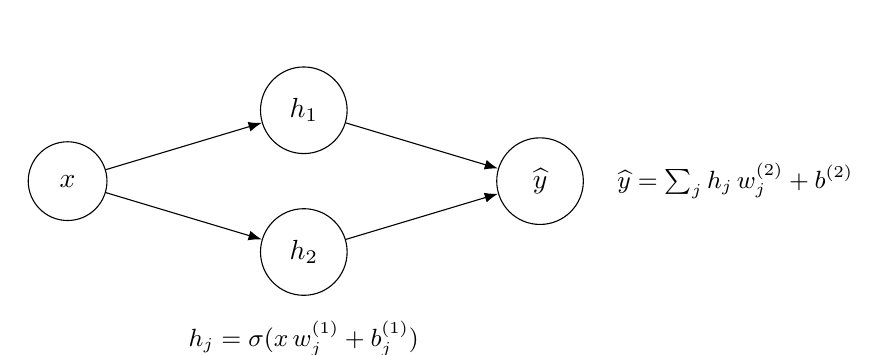
\begin{tikzpicture}[>=Latex]
\node[draw,circle,minimum size=10mm] (x) at (0,0) {$x$};
\node[draw,circle,minimum size=11mm] (h1) at (3,0.9) {$h_1$};
\node[draw,circle,minimum size=11mm] (h2) at (3,-0.9) {$h_2$};
\node[draw,circle,minimum size=11mm] (y) at (6,0) {$\widehat y$};
\foreach \h in {h1,h2} { \draw[->] (x) -- (\h); \draw[->] (\h) -- (y); }
\node[below=2mm of h2] {\small $h_j=\sigmoid(x\,w^{(1)}_j+b^{(1)}_j)$};
\node[right=3mm of y] {\small $\widehat y=\sum_j h_j\,w^{(2)}_j+b^{(2)}$};
\end{tikzpicture}
\end{center}

데이터는 $x$축 위에 순서대로 놓인 네 개의 class $t\in\{0,1,2,3\}$이다.
class 번호를 target 값으로 두고 MSE로 학습한 뒤,
출력 $\widehat y$를 가장 가까운 정수로 반올림하여 class를 예측한다.
target이 계단 모양이므로,
7절에서 본 것처럼 여러 sigmoid를 조합해야 표현할 수 있다.

\subsection{Step 1. 데이터와 parameter}

$N$개의 데이터를 한 줄에 하나씩 쌓아 \textbf{데이터 행렬}로 만든다.
\texttt{reshape(-1, 1)}은 길이 $N$인 1차원 배열을 $N\times1$ 행렬(열벡터)로 바꾼다.

\begin{lstlisting}
import numpy as np
import matplotlib.pyplot as plt

np.random.seed(0)

# data: N rows = N samples, 4 classes ordered along x
x = np.array([-5, -4, -3, -2, -1, 0, 1, 2, 3, 4, 5, 6],
             dtype=float).reshape(-1, 1)       # X: (N, 1)
t = np.array([ 0,  0,  0,  0,  1, 1, 1, 2, 2, 3, 3, 3],
             dtype=float).reshape(-1, 1)       # T: (N, 1)
N = x.shape[0]

m = 2   # number of hidden neurons

# parameters (row-vector convention: a = x W1 + b1,  y = h W2 + b2)
W1 = np.random.randn(1, m) * 0.5 + 0.1   # (1, m)
b1 = np.random.randn(1, m) * 0.5 + 0.1   # (1, m)
W2 = np.random.randn(m, 1) * 0.5         # (m, 1)
b2 = np.random.randn(1, 1) * 0.5         # (1, 1)

learning_rate = 0.2
epochs = 20000

def sigmoid(a):
    return 1.0 / (1.0 + np.exp(-a))
\end{lstlisting}

\subsection{Step 2. Forward}

전체 데이터를 한 번에 network에 흘려보낸다.

\begin{lstlisting}
a = x @ W1 + b1      # (N,1) @ (1,m) + (1,m) -> (N, m)
h = sigmoid(a)       # (N, m)
y = h @ W2 + b2      # (N,m) @ (m,1) + (1,1) -> (N, 1)

error = y - t        # (N, 1)
loss = np.mean(error**2)
\end{lstlisting}

데이터 $i$ 하나에 대해서는 6절과 똑같이
\[
a_{ij}=x_i\,w^{(1)}_j+b^{(1)}_j,
\qquad
h_{ij}=\sigmoid(a_{ij}),
\qquad
y_i=\sum_{j=1}^{m}h_{ij}\,w^{(2)}_j+b^{(2)},
\qquad
e_i=y_i-t_i
\]
를 계산하고, loss는 $L=\frac1N\sum_{i=1}^{N}e_i^2$이다.
데이터 행렬
\[
X=
\begin{bmatrix}
x_1\\ \vdots\\ x_N
\end{bmatrix}\in\R^{N\times1},
\qquad
T=
\begin{bmatrix}
t_1\\ \vdots\\ t_N
\end{bmatrix}\in\R^{N\times1}
\]
로 한꺼번에 쓰면
\[
A=XW^{(1)}+\mathbf 1\,\vect{b}^{(1)},
\qquad
H=\sigmoid(A),
\qquad
\vect{y}=H\vect{w}^{(2)}+\mathbf 1\,b^{(2)},
\qquad
\vect{e}=\vect{y}-T
\]
이다.
$A,H\in\R^{N\times m}$의 $i$번째 행이 6.2절의 $\vect{a}$, $\vect{h}$, 즉 데이터 $i$의 hidden layer이다.
($\mathbf 1\in\R^{N\times1}$은 모든 성분이 $1$인 벡터이며,
NumPy에서는 \texttt{+ b1}, \texttt{+ b2}의 broadcasting이 이 역할을 한다.)

\subsection{Step 3. Backward --- local derivative를 그대로 코드로 쓰기}

\begin{lstlisting}
# Row i of every array below belongs to sample i.
# So each row is exactly the single-sample backprop,
# computed for all N samples at the same time.

# ---- output layer:  y_i = sum_j h_ij * w2_j + b2 ----
dL_dy = 2.0 * error / N       # (N, 1)  L = mean(e**2) -> 2 e_i / N

# W2, b2 are SHARED by all N samples -> sum of contributions
dL_dW2 = h.T @ dL_dy                           # (m,N)@(N,1) -> (m, 1)
dL_db2 = np.sum(dL_dy, axis=0, keepdims=True)  # (1, 1)

# ---- back to the hidden layer:  dy_i/dh_ij = w2_j ----
dL_dh = dL_dy @ W2.T          # (N,1)@(1,m) -> (N, m)

# ---- through the sigmoid (elementwise):  dh/da = h (1 - h) ----
dL_da = dL_dh * h * (1.0 - h) # (N, m)

# W1, b1 are SHARED by all N samples -> sum of contributions
dL_dW1 = x.T @ dL_da                           # (1,N)@(N,m) -> (1, m)
dL_db1 = np.sum(dL_da, axis=0, keepdims=True)  # (1, m)

# Because dL_dy already contains 1/N, these sums are the
# AVERAGE of the per-sample gradients.
\end{lstlisting}

데이터 $i$ 하나에 대한 backward는 출력에서 입력 방향으로
local derivative를 차례로 곱하는 것이다:
\[
\delta_i
:=
\frac{\partial L}{\partial y_i}
=
\frac{2e_i}{N},
\qquad
\frac{\partial L}{\partial h_{ij}}
=
\delta_i\,
\underbrace{\frac{\partial y_i}{\partial h_{ij}}}_{w^{(2)}_j},
\qquad
\delta_{ij}
:=
\frac{\partial L}{\partial a_{ij}}
=
\frac{\partial L}{\partial h_{ij}}\,
\underbrace{\frac{\partial h_{ij}}{\partial a_{ij}}}_{h_{ij}(1-h_{ij})}.
\]

\begin{thinkbox}[기호 $\delta$와 $\Delta$: 각 node에 도착한 gradient]
backpropagation에서 $\delta$는 관례적으로
``loss $L$을 어떤 node의 값으로 미분한 것'', 즉
\textbf{출력 쪽에서 그 node까지 거꾸로 전달되어 온 gradient}를 나타낸다.
이 값만 알면 그 node로 들어오는 parameter의 gradient는
local derivative 하나를 더 곱해서 바로 얻을 수 있다.

\begin{itemize}[leftmargin=1.8em]
\item $\delta_i=\dfrac{\partial L}{\partial y_i}$:
데이터 $i$의 \textbf{출력 node} $y_i$에 도착한 gradient (스칼라).
\item $\delta_{ij}=\dfrac{\partial L}{\partial a_{ij}}$:
데이터 $i$의 \textbf{$j$번째 hidden neuron의 입력} $a_{ij}$
(activation을 통과하기 전 값)에 도착한 gradient (스칼라).
\end{itemize}

이들을 $N$개의 데이터에 대해 모아 행렬로 쓴 것이
\[
\boldsymbol\delta
=
\begin{bmatrix}
\delta_1\\ \vdots\\ \delta_N
\end{bmatrix}
\in\R^{N\times1},
\qquad
\Delta
=
\begin{bmatrix}
\delta_{11} & \cdots & \delta_{1m}\\
\vdots & \ddots & \vdots\\
\delta_{N1} & \cdots & \delta_{Nm}
\end{bmatrix}
\in\R^{N\times m}
\]
이다. ($\Delta$는 대문자 delta이며, 여기서는 ``변화량''이 아니라 $\delta_{ij}$를 모은 행렬을 뜻한다.)
$\Delta$의 $i$번째 행은 데이터 $i$의 hidden layer 전체에 도착한 gradient이다.

\begin{center}
\begin{tabular}{@{}lll@{}}
\toprule
기호 & 의미 & 코드 \\
\midrule
$\boldsymbol\delta\in\R^{N\times1}$ & $\partial L/\partial \vect{y}$ (출력 node) & \texttt{dL\_dy} \\
$\Delta\in\R^{N\times m}$ & $\partial L/\partial A$ (hidden neuron의 입력) & \texttt{dL\_da} \\
\bottomrule
\end{tabular}
\end{center}
\end{thinkbox}

parameter에 대해서는
\[
\frac{\partial L}{\partial w^{(2)}_j}=\sum_{i=1}^{N}h_{ij}\,\delta_i,
\qquad
\frac{\partial L}{\partial b^{(2)}}=\sum_{i=1}^{N}\delta_i,
\qquad
\frac{\partial L}{\partial w^{(1)}_j}=\sum_{i=1}^{N}x_i\,\delta_{ij},
\qquad
\frac{\partial L}{\partial b^{(1)}_j}=\sum_{i=1}^{N}\delta_{ij}
\]
이다.
이를 행렬로 쓰면 ($\odot$는 성분별 곱)
\[
\boxed{
\begin{gathered}
\text{output layer:}\quad
\boldsymbol\delta=\tfrac{2}{N}\vect{e},
\qquad
\frac{\partial L}{\partial \vect{w}^{(2)}}=H^{\!\top}\boldsymbol\delta,
\qquad
\frac{\partial L}{\partial b^{(2)}}=\mathbf 1^{\!\top}\boldsymbol\delta
\\[6pt]
\text{hidden layer:}\quad
\Delta=\bigl(\boldsymbol\delta\,(\vect{w}^{(2)})^{\!\top}\bigr)\odot H\odot(1-H),
\qquad
\frac{\partial L}{\partial W^{(1)}}=X^{\!\top}\Delta,
\qquad
\frac{\partial L}{\partial \vect{b}^{(1)}}=\mathbf 1^{\!\top}\Delta
\end{gathered}
}
\]
이며, 코드의 \texttt{h.T @ dL\_dy}, \texttt{dL\_dy @ W2.T}, \texttt{x.T @ dL\_da},
\texttt{np.sum(..., axis=0)}가 정확히 이것이다.

\begin{remarkbox}[왜 bias의 gradient는 합(sum)인가?]
앞 절의 backpropagation은 데이터 \textbf{하나}에 대한 계산이었다.
코드에서는 $N$개의 데이터를 한 번에 흘려보내므로,
\texttt{dL\_dy}, \texttt{dL\_da}의 $i$번째 행이 곧 데이터 $i$ 하나에 대한 $\delta_i$, $\delta_{ij}$이다.

그런데 parameter는 데이터마다 따로 있는 것이 아니라
\textbf{모든 데이터가 공유}한다. 예를 들어 출력층의 bias는
\[
y_1=\textstyle\sum_j h_{1j}w^{(2)}_j+b^{(2)},\quad
\ldots,\quad
y_N=\sum_j h_{Nj}w^{(2)}_j+b^{(2)}
\]
처럼 $y_1,\ldots,y_N$ 모두에 들어간다
(forward에서 $b^{(2)}$가 $N$개의 행으로 broadcast된다).
따라서 chain rule에 의해 각 경로의 기여를 모두 더해야 한다:
\[
\frac{\partial L}{\partial b^{(2)}}
=
\sum_{i=1}^{N}
\frac{\partial L}{\partial y_i}\,
\underbrace{\frac{\partial y_i}{\partial b^{(2)}}}_{1}
=
\sum_{i=1}^{N}\delta_i .
\]
$\vect{b}^{(1)}$, $W^{(1)}$, $\vect{w}^{(2)}$도 같은 이유로 데이터에 대한 합이 되고,
weight의 경우 그 합을 행렬곱 $X^{\!\top}\Delta$, $H^{\!\top}\boldsymbol\delta$로 한 번에 계산한다.
$\boldsymbol\delta$ 안에 $1/N$이 들어 있으므로 이 합은 곧
\textbf{데이터별 gradient의 평균}이며,
parameter는 epoch마다 한 번 업데이트된다 (full-batch gradient descent).
\end{remarkbox}

\subsection{Step 4. Parameter update}

\begin{lstlisting}
W1 -= learning_rate * dL_dW1
b1 -= learning_rate * dL_db1
W2 -= learning_rate * dL_dW2
b2 -= learning_rate * dL_db2
\end{lstlisting}

즉, 모든 parameter $\theta\in\{W^{(1)},\vect{b}^{(1)},\vect{w}^{(2)},b^{(2)}\}$에 대해
\[
\theta\leftarrow\theta-\eta\frac{\partial L}{\partial \theta}.
\]

\subsection{Step 5. 전체 training loop}

\begin{lstlisting}
import os
import numpy as np
import matplotlib.pyplot as plt

np.random.seed(0)
os.makedirs("figures", exist_ok=True)   # folder for saved figures

x = np.array([-5, -4, -3, -2, -1, 0, 1, 2, 3, 4, 5, 6],
             dtype=float).reshape(-1, 1)       # (N, 1)
t = np.array([ 0,  0,  0,  0,  1, 1, 1, 2, 2, 3, 3, 3],
             dtype=float).reshape(-1, 1)       # (N, 1)
N = x.shape[0]

m = 2
W1 = np.random.randn(1, m) * 0.5 + 0.1
b1 = np.random.randn(1, m) * 0.5 + 0.1
W2 = np.random.randn(m, 1) * 0.5
b2 = np.random.randn(1, 1) * 0.5

learning_rate = 0.2
epochs = 20000
loss_history = []

def sigmoid(a):
    return 1.0 / (1.0 + np.exp(-a))

for epoch in range(epochs):

    # -----------------------------
    # 1. Forward (all N samples at once)
    # -----------------------------
    a = x @ W1 + b1            # (N, m)
    h = sigmoid(a)             # (N, m)
    y = h @ W2 + b2            # (N, 1)

    error = y - t
    loss = np.mean(error**2)

    # -----------------------------
    # 2. Backward (row i = single-sample backprop of sample i)
    # -----------------------------
    dL_dy = 2.0 * error / N                        # (N, 1)
    dL_dW2 = h.T @ dL_dy                           # (m, 1)  sum over samples
    dL_db2 = np.sum(dL_dy, axis=0, keepdims=True)  # (1, 1)  sum over samples

    dL_dh = dL_dy @ W2.T                           # (N, m)
    dL_da = dL_dh * h * (1.0 - h)                  # (N, m)
    dL_dW1 = x.T @ dL_da                           # (1, m)  sum over samples
    dL_db1 = np.sum(dL_da, axis=0, keepdims=True)  # (1, m)  sum over samples

    # -----------------------------
    # 3. Gradient descent (one update per epoch)
    # -----------------------------
    W1 -= learning_rate * dL_dW1
    b1 -= learning_rate * dL_db1
    W2 -= learning_rate * dL_dW2
    b2 -= learning_rate * dL_db2

    loss_history.append(loss)

    if epoch % 2000 == 0:
        print(f"epoch={epoch:5d}, loss={loss:.6f}")

print("W1 =", W1)
print("b1 =", b1)
print("W2 =", W2.ravel())
print("b2 =", b2)

# prediction curve
x_plot = np.linspace(-7.0, 8.0, 300).reshape(-1, 1)   # (300, 1)
h_plot = sigmoid(x_plot @ W1 + b1)                    # (300, m)
y_plot = h_plot @ W2 + b2                             # (300, 1)

plt.figure(figsize=(10, 4))
plt.subplot(1, 2, 1)
plt.plot(x, t, "ro", label="data")
plt.plot(x_plot, y_plot, "k", label="network output")
plt.xlabel("x")
plt.ylabel("y")
plt.title("2-Layer Neural Network")
plt.legend()
plt.grid(True)

plt.subplot(1, 2, 2)
plt.plot(loss_history)
plt.xlabel("epoch")
plt.ylabel("MSE loss")
plt.title("Cost History")
plt.grid(True)
plt.tight_layout()
plt.savefig("figures/lab_fit_and_cost.png", dpi=200)
plt.show()

# what does each hidden neuron do?
plt.figure(figsize=(10, 4))
plt.subplot(1, 2, 1)
for j in range(m):
    plt.plot(x_plot, h_plot[:, j], "--", label=f"h_{j+1}")
plt.title("hidden layer outputs")
plt.legend()
plt.grid(True)

plt.subplot(1, 2, 2)
for j in range(m):
    plt.plot(x_plot, h_plot[:, j] * W2[j, 0], "--", label=f"h_{j+1} * w2_{j+1}")
plt.plot(x_plot, y_plot, "k", label="y = sum + b2")
plt.title("output layer")
plt.legend()
plt.grid(True)
plt.tight_layout()
plt.savefig("figures/lab_hidden_units.png", dpi=200)
plt.show()
\end{lstlisting}

학습 후에는 network 출력 $\widehat y(x)$가 데이터의 계단 모양을 따라가는 곡선이 된다.
그림은 \texttt{figures} 폴더에 \texttt{png} 파일로도 저장된다.

\IfFileExists{figures/lab_fit_and_cost.png}{%
\begin{center}
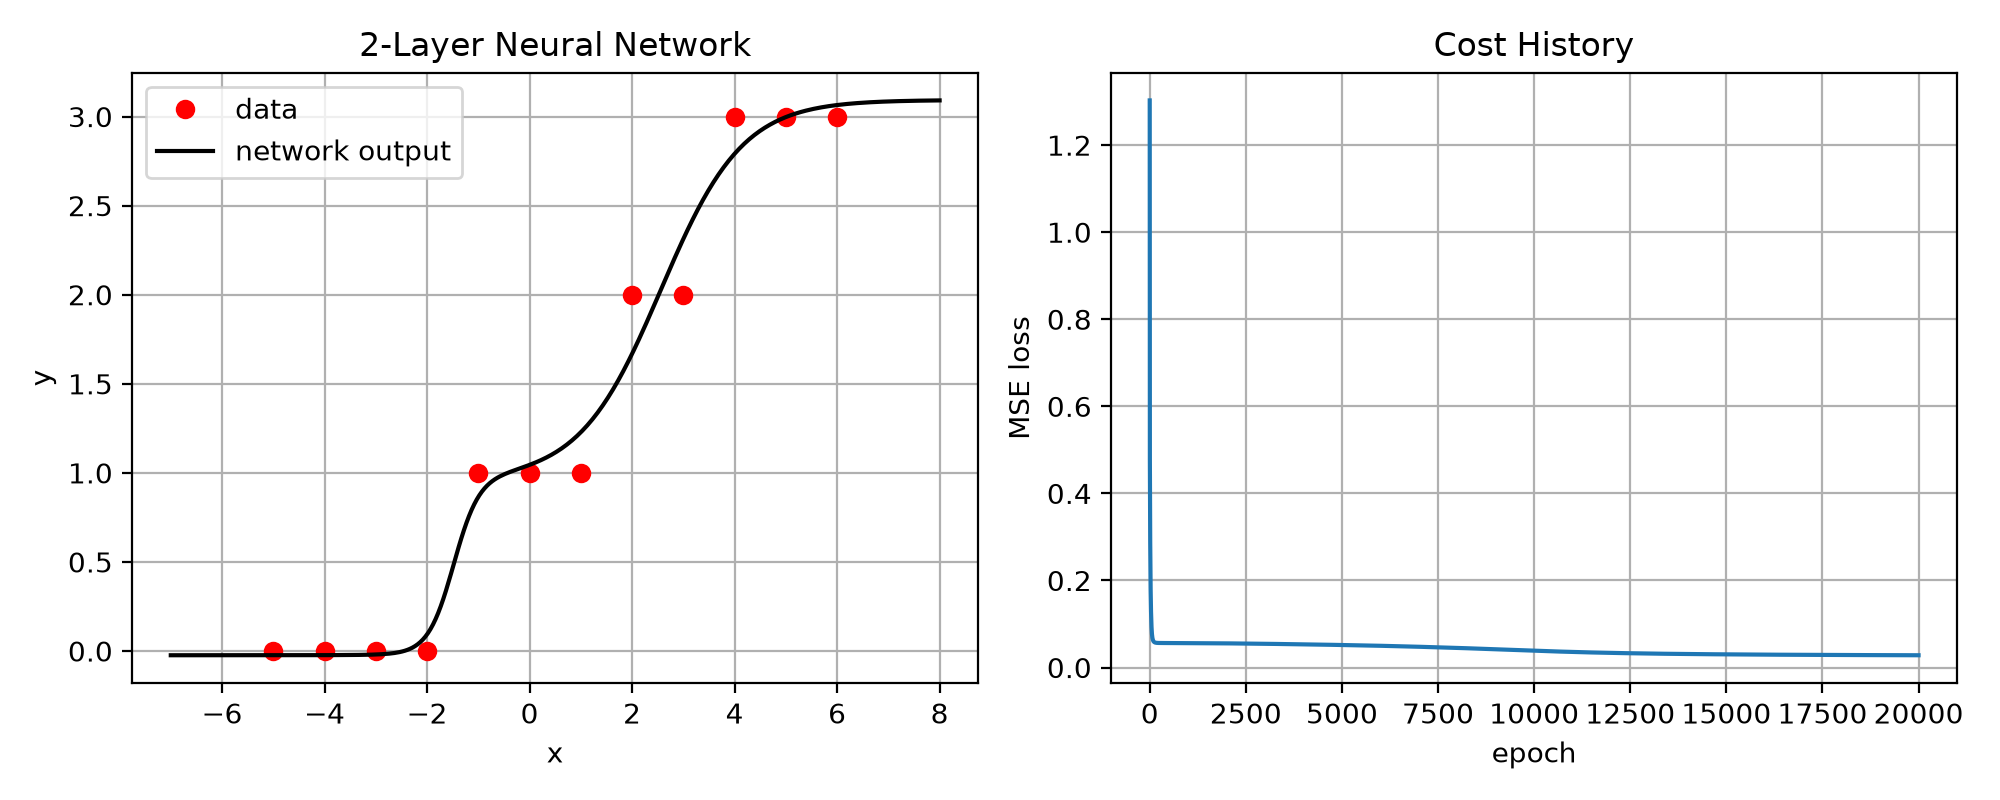
\includegraphics[width=\textwidth]{figures/lab_fit_and_cost.png}

\small 학습된 network의 출력(왼쪽)과 cost history(오른쪽)
\end{center}
}{%
\begin{center}
\fbox{\parbox{0.8\textwidth}{\centering\small
[그림 자리] \texttt{figures/lab\_fit\_and\_cost.png}\\
Step 5 코드를 실행하면 생성된다.}}
\end{center}
}

아래 그림에서 각 hidden neuron의 출력 $h_j(x)$는
서로 다른 위치 $-b^{(1)}_j/w^{(1)}_j$와 기울기를 가진 S-shaped curve이고,
출력층은 이들을 $w^{(2)}_j$배 하여 더한 뒤 $b^{(2)}$만큼 평행이동한다.

\IfFileExists{figures/lab_hidden_units.png}{%
\begin{center}
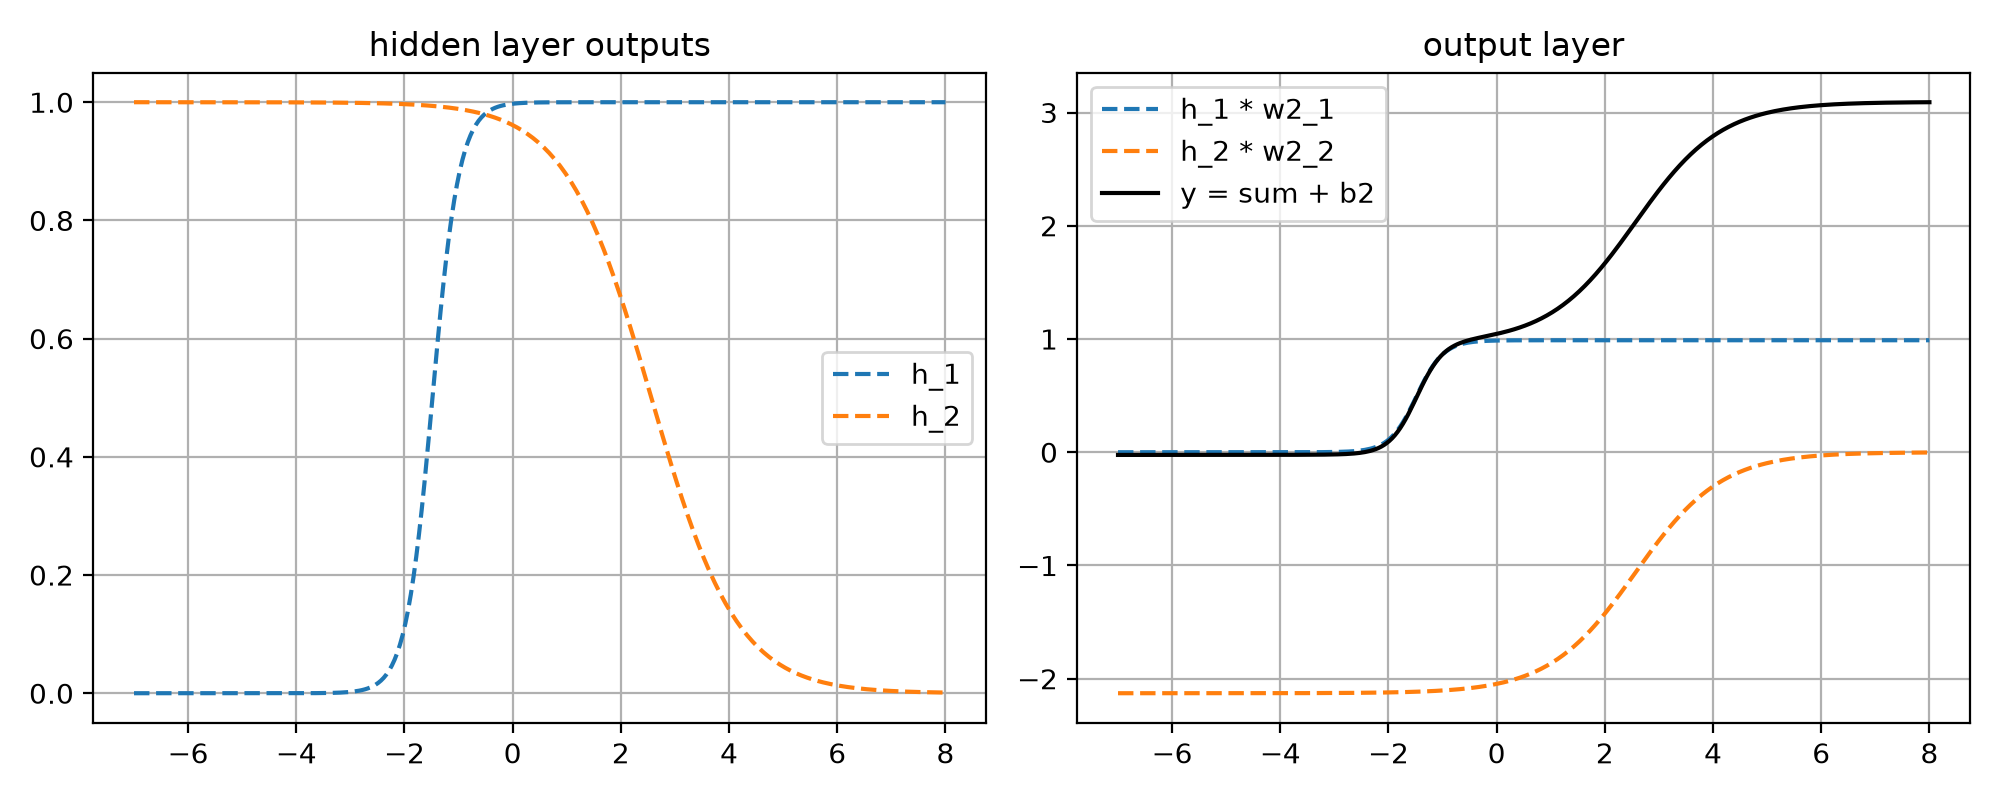
\includegraphics[width=\textwidth]{figures/lab_hidden_units.png}

\small hidden layer의 출력 $h_j(x)$(왼쪽)와 출력층에서의 조합 $h_j(x)\,w^{(2)}_j$(오른쪽)
\end{center}
}{%
\begin{center}
\fbox{\parbox{0.8\textwidth}{\centering\small
[그림 자리] \texttt{figures/lab\_hidden\_units.png}\\
Step 5 코드를 실행하면 생성된다.}}
\end{center}
}

\begin{thinkbox}[관찰해 보자]
데이터의 계단은 세 개이지만 hidden neuron은 두 개뿐이다.
학습된 두 neuron은 대체로 다음과 같이 역할을 나눈다.
\begin{itemize}[leftmargin=1.8em]
\item 한 neuron은 $x\approx-1.5$ 근처에서 \textbf{가파르게} 전이하여 높이 $1$의 첫 번째 계단을 만든다.
\item 다른 neuron은 $x\approx2.5$ 근처를 중심으로 \textbf{완만하게} 전이하여,
높이 약 $2$의 S-shaped curve 하나로 위쪽 두 계단($1\to2\to3$)을 함께 따라간다.
\end{itemize}
데이터가 정수 위치에만 있으므로, 완만한 sigmoid 하나로도 두 계단을 충분히 지나갈 수 있는 것이다.
즉 7절처럼 계단마다 sigmoid를 하나씩 배정하지 않아도 된다.
\texttt{m}을 $3$, $5$로 늘리면 training loss는 조금 줄지만 곡선에 불필요한 굴곡이 생기는지 관찰하라.
(과제 2와 7.3절: 표현 가능성과 학습 가능성은 다른 문제이다.)
\end{thinkbox}

\subsection{Step 6. 분류 결과 확인}

\begin{lstlisting}
a = x @ W1 + b1
h = sigmoid(a)
y = h @ W2 + b2

# nearest class index (0, 1, 2, 3)
prediction = np.clip(np.rint(y), 0, 3).astype(int)

print("network output =", np.round(y.ravel(), 3))
print("prediction     =", prediction.ravel())
print("target         =", t.ravel().astype(int))
\end{lstlisting}

\subsection{Step 7. Hidden neurons가 만드는 basis function 관찰}

이번에는 training을 하지 않고,
여러 sigmoid를 조합하면 복잡한 함수를 만들 수 있다는 사실만 확인해보자.

\begin{lstlisting}
import numpy as np
import matplotlib.pyplot as plt

def sigmoid(a):
    return 1.0 / (1.0 + np.exp(-a))

x = np.linspace(-0.5, 4.5, 500)

k = 20.0

# four approximate rectangular bumps
r0 = sigmoid(k*(x-0)) - sigmoid(k*(x-1))
r1 = sigmoid(k*(x-1)) - sigmoid(k*(x-2))
r2 = sigmoid(k*(x-2)) - sigmoid(k*(x-3))
r3 = sigmoid(k*(x-3)) - sigmoid(k*(x-4))

# left-endpoint values of f(x)=x^2+2
f_approx = 2*r0 + 3*r1 + 6*r2 + 11*r3
f_true = x**2 + 2

plt.figure(figsize=(7, 4))
plt.plot(x, f_true, label="f(x)=x^2+2")
plt.plot(x, f_approx, label="sigmoid combination")
plt.xlim(0, 4)
plt.xlabel("x")
plt.ylabel("y")
plt.legend()
plt.grid(True)
plt.show()
\end{lstlisting}

여기서 각 $r_j$는 sigmoid 두 개의 차로 만든 approximate rectangular bump이고,
이들을 서로 다른 계수로 더하여 $x^2+2$를 거칠게 근사하였다.

hidden neurons의 수를 늘리고 interval을 더 잘게 나누면
더 정밀한 approximation을 만들 수 있다.

% =================================================
\section{이번 주의 핵심 정리}
% =================================================

\begin{keybox}[핵심 구조]
하나의 neuron:
\[
\boxed{
a=\vect{w}\T\vect{x}+b,
\qquad
z=\phi(a)
}
\]

Activation의 역할:
\[
\boxed{
\text{network에 nonlinearity를 넣는다}
}
\]

Single sigmoid neuron:
\[
\boxed{
z=\sigmoid(wx+b)
}
\]
는 하나의 transition을 표현한다.

Hidden layer:
\[
\boxed{
\widehat y(x)
=
\sum_{j=1}^{m}
w_j^{(2)}
\phi(w_j^{(1)}x+b_j^{(1)})
+b^{(2)}
}
\]
는 여러 nonlinear building blocks를 조합한다.

Backpropagation:
\[
\boxed{
\text{뒤쪽 gradient}
\times
\text{local derivative}
\longrightarrow
\text{앞쪽 gradient}
}
\]

Universal approximation:
\[
\boxed{
\text{충분히 많은 hidden neurons}
\Rightarrow
\text{매우 풍부한 함수 표현력}
}
\]
\end{keybox}

% =================================================
\section{연습문제}
% =================================================

\begin{enumerate}[label=\arabic*.]

\item
\[
a=2x-1,
\qquad
z=\sigmoid(a)
\]
에서 $x=1$일 때 $a$, $z$, $dz/da$, $dz/dx$를 계산하라.

\item 하나의 neuron
\[
a=w_1x_1+w_2x_2+b,
\qquad
z=\sigmoid(a)
\]
에 대해
\[
\nabla_{\vect{w}}z
\]
를 구하라.

\item sigmoid neuron에서 $w>0$일 때
\[
z(x)=\sigmoid(wx+b)=0.5
\]
가 되는 $x$를 구하고, $w$와 $b$가 decision boundary에 어떤 영향을 주는지 설명하라.

\item
\[
\ell=(z-t)^2,\qquad
z=\sigmoid(wx+b)
\]
에 대해 computational graph를 그리고
\[
\frac{\partial\ell}{\partial w},
\qquad
\frac{\partial\ell}{\partial b}
\]
를 local derivative의 곱으로 유도하라.

\item 활성화 함수가 identity,
\[
\phi(a)=a,
\]
라고 하자. 두 affine layer
\[
\vect{h}=W_1\vect{x}+\vect{b}_1,
\qquad
\vect{y}=W_2\vect{h}+\vect{b}_2
\]
를 하나의 affine layer로 합칠 수 있음을 보이라.

\item 하나의 sigmoid neuron으로
\[
(0,1,1,1,0)
\]
과 같이 가운데에서만 class $1$인 1차원 classification pattern을 완벽하게 표현하기 어려운 이유를 설명하라.

\item
\[
r_{a,b}(x)
=
\sigmoid(k(x-a))-\sigmoid(k(x-b))
\]
에서 $k$가 매우 커질 때 함수의 모양이 어떻게 변하는지 설명하라.

\item Universal Approximation Theorem이
``gradient descent가 항상 좋은 solution을 찾는다''는 것을 의미하지 않는 이유를 설명하라.

\end{enumerate}

% =================================================
\section{과제}
% =================================================

과제 1은 hidden layer가 있는 network의 순전파와 역전파를 \textbf{손으로} 끝까지 계산해 보는 문제이고,
과제 2는 3차시 실습 코드로 network를 \textbf{설계하고 훈련}해 보는 문제이다.

\subsection*{과제 1. 은닉층이 있는 신경망의 역전파를 손으로 계산하기}

다음과 같은 데이터가 주어졌다고 하자.

\begin{center}
\begin{minipage}{0.36\textwidth}
\centering
\begin{tabular}{|c|c|c|}
\hline
\rowcolor{cyan!25}
$i$ & $x$ & $t$ \\
\hline
0 & $-2$ & 0 \\ \hline
1 & $-1$ & 0 \\ \hline
2 & $0$ & 1 \\ \hline
3 & $1$ & 1 \\ \hline
4 & $2$ & 1 \\ \hline
5 & $3$ & 1 \\ \hline
6 & $4$ & 0 \\ \hline
7 & $5$ & 0 \\ \hline
\end{tabular}
\end{minipage}
\hfill
\begin{minipage}{0.58\textwidth}
\centering
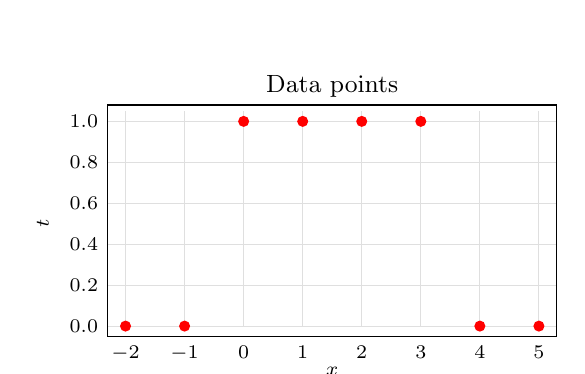
\begin{tikzpicture}[x=0.75cm,y=2.6cm]
\foreach \gx in {-2,...,5} \draw[gray!25] (\gx,0) -- (\gx,1.05);
\foreach \gy in {0,0.2,0.4,0.6,0.8,1.0} \draw[gray!25] (-2.3,\gy) -- (5.3,\gy);
\draw (-2.3,-0.05) rectangle (5.3,1.08);
\foreach \gx in {-2,...,5} \node[below,font=\scriptsize] at (\gx,-0.05) {$\gx$};
\foreach \gy in {0.0,0.2,0.4,0.6,0.8,1.0} \node[left,font=\scriptsize] at (-2.3,\gy) {\gy};
\foreach \px/\pt in {-2/0,-1/0,0/1,1/1,2/1,3/1,4/0,5/0}
  \fill[red] (\px,\pt) circle (2pt);
\node[font=\small] at (1.5,1.17) {Data points};
\node[font=\scriptsize] at (1.5,-0.22) {$x$};
\node[font=\scriptsize,rotate=90] at (-3.4,0.5) {$t$};
\end{tikzpicture}
\end{minipage}
\end{center}

은닉층이 1층이고 두 개의 노드를 갖는 함수로 주어진 데이터를 회귀하고자 한다.

\begin{center}
\begin{tikzpicture}[>=Latex,
  nd/.style={draw,circle,minimum size=8mm,inner sep=0pt},
  bias/.style={draw,circle,minimum size=8mm,inner sep=0pt,fill=blue!55!black,text=white},
  tag/.style={fill=red!80!black,text=white,font=\small,inner sep=2pt},
  boxlabel/.style={draw=blue!60!black,fill=cyan!20,font=\small,inner sep=3pt}]
% frames
\draw (-0.7,-3.7) rectangle (7.6,2.7);
\draw (7.9,-3.7) rectangle (12.6,2.7);
% input layer
\node[bias] (one1) at (0,1.7) {$1$};
\node[nd] (x) at (0,-0.6) {$x$};
% hidden layer
\draw (3.6,0.8) circle (0.95);
\draw (3.6,-1.4) circle (0.95);
\node[nd] (a1) at (3.15,0.8) {$a_1$};
\node[nd] (z1) at (4.05,0.8) {$z_1$};
\node[nd] (a2) at (3.15,-1.4) {$a_2$};
\node[nd] (z2) at (4.05,-1.4) {$z_2$};
% output layer
\node[bias] (one2) at (3.6,2.25) {$1$};
\node[nd] (y) at (6.4,-0.1) {$y$};
% loss
\node[nd] (mt) at (9.6,1.2) {$-t$};
\node[nd] (e) at (9.6,-0.1) {$e$};
\node[nd] (l) at (11.6,-0.1) {$l$};
% arrows
\draw[->,blue!50!black] (one1) -- (a1);
\draw[->,blue!50!black] (one1) -- (a2);
\draw[->,blue!50!black] (x) -- (a1);
\draw[->,blue!50!black] (x) -- (a2);
\draw[->] (a1) -- (z1);
\draw[->] (a2) -- (z2);
\draw[->,blue!50!black] (z1) -- (y);
\draw[->,blue!50!black] (z2) -- (y);
\draw[->,blue!50!black] (one2) -- (y);
\draw[->,blue!50!black] (y) -- (e);
\draw[->,blue!50!black] (mt) -- (e);
\draw[->,blue!50!black] (e) -- (l);
% labels
\node[tag] at (1.55,-1.15) {$W^{(1)},B^{(1)}$};
\node[tag] at (5.55,-1.15) {$W^{(2)},B^{(2)}$};
\node[font=\small] at (0,-1.35) {입력층};
\node[font=\small] at (3.6,-2.75) {은닉층};
\node[font=\small] at (6.4,0.6) {출력층};
\node[boxlabel] at (3.45,-3.3) {신경망 입출력};
\node[boxlabel] at (10.25,-3.3) {손실 함수};
\end{tikzpicture}

\small 그림 4
\end{center}

활성화함수 \textcolor{red}{$h(x)=\max(0,x)$ (ReLU)}일 때, 각 노드에 나타나는 변수들을
\[
\begin{cases}
a_1=xw^{(1)}_1+b^{(1)}_1\\[2pt]
a_2=xw^{(1)}_2+b^{(1)}_2
\end{cases},
\qquad
\begin{cases}
z_1=h(a_1)\\[2pt]
z_2=h(a_2)
\end{cases},
\qquad
y=z_1w^{(2)}_1+z_2w^{(2)}_2+b^{(2)}
\]
로 정의하면
\[
y=w^{(2)}_1h\bigl(w^{(1)}_1x+b^{(1)}_1\bigr)+w^{(2)}_2h\bigl(w^{(1)}_2x+b^{(1)}_2\bigr)+b^{(2)}
\]
이고, 가중치와 편이와 은닉층의 변수를 행렬로
\[
W^{(1)}_{1\times2}=\bigl(w^{(1)}_1,w^{(1)}_2\bigr),\quad
B^{(1)}_{1\times2}=\bigl(b^{(1)}_1,b^{(1)}_2\bigr),\quad
W^{(2)}_{2\times1}=
\begin{pmatrix}
w^{(2)}_1\\ w^{(2)}_2
\end{pmatrix},\quad
B^{(2)}_{1\times1}=\bigl(b^{(2)}\bigr)
\]
\[
A=(a_1,a_2),\quad Z=(z_1,z_2)
\]
로 정의하면, 신경망은 다음과 같은 단계를 따라 출력 $y$를 계산한다.
\[
A=(x)_{1\times1}W^{(1)}+B^{(1)},\quad
Z=h(A),\quad
y=ZW^{(2)}+B^{(2)}
\]

신경망의 출력 $y$와 실제 데이터 $t$의 차이인 오차를 $e=y-t$이라 정의하고, 제곱 오차를 $l=e^2$이라 하자.
모든 데이터에 대한 평균제곱 손실함수(MSE)는
\[
L\bigl(W^{(1)},B^{(1)},W^{(2)},B^{(2)}\bigr)=\frac1N\sum_{i=0}^{N-1}l_i
\]
이다.

\begin{remarkbox}[ReLU의 도함수]
ReLU의 도함수는
\[
h'(x)=\begin{cases}1,&x>0\\0,&x<0\end{cases}
\]
이다. 즉 입력이 양수인 노드는 gradient를 그대로 통과시키고,
입력이 음수인 노드는 gradient를 $0$으로 막는다.
(꺾이는 점 $x=0$에서는 미분이 정의되지 않으므로 보통 $h'(0)=0$으로 약속한다.
NumPy 코드의 \texttt{np.where(a > 0, 1, 0)}과 같다.)
\end{remarkbox}

데이터 $(x_3,t_3)=(1,1)$와 가중치와 편이의 초깃값
\[
W^{(1)}_0=(1,0),\quad
B^{(1)}_0=(0,1),\quad
W^{(2)}_0=
\begin{pmatrix}
3\\ 2
\end{pmatrix},\quad
B^{(2)}_0=0
\]
에 대하여

\begin{enumerate}[leftmargin=2.2em]
\item[가.] 순전파로 정해지는 변수값 $A,Z,y,e,l$의 값을 구하여라.
\item[나.] 역전파로 정해지는 편미분
\[
\frac{\partial l}{\partial e},\
\frac{\partial l}{\partial y},\
\frac{\partial l}{\partial W^{(2)}_0},\
\frac{\partial l}{\partial B^{(2)}_0},\
\frac{\partial l}{\partial Z},\
\frac{\partial l}{\partial A},\
\frac{\partial l}{\partial W^{(1)}_0},\
\frac{\partial l}{\partial B^{(1)}_0},\
\frac{\partial l}{\partial x}
\]
의 값을 구하여라.
\item[다.] $\alpha=0.01$일 때, 경사하강법을 적용하여
\[
\begin{cases}
W^{(1)}_1=W^{(1)}_0-\alpha\dfrac{\partial l}{\partial W^{(1)}_0}\\[10pt]
B^{(1)}_1=B^{(1)}_0-\alpha\dfrac{\partial l}{\partial B^{(1)}_0}\\[10pt]
W^{(2)}_1=W^{(2)}_0-\alpha\dfrac{\partial l}{\partial W^{(2)}_0}\\[10pt]
B^{(2)}_1=B^{(2)}_0-\alpha\dfrac{\partial l}{\partial B^{(2)}_0}
\end{cases}
\]
$W^{(1)}_1,B^{(1)}_1,W^{(2)}_1,B^{(2)}_1$를 구하여라.
\item[라.] 만약 초깃값이 $B^{(1)}_0=(0,-1)$이었다면 (나머지 초깃값과 데이터는 같다),
나.의 편미분 중 어떤 값이 $0$이 되는가?
이때 두 번째 은닉 노드의 가중치 $w^{(1)}_2$, 편이 $b^{(1)}_2$, 가중치 $w^{(2)}_2$는
경사하강법으로 업데이트되는가?
만약 \textbf{모든} 데이터에 대해 $a_2<0$이라면 학습이 진행되어도 어떤 일이 일어나겠는가?
\end{enumerate}

\subsection*{과제 2. 신경망 설계와 훈련 실험}

3차시 실습 Step 5의 코드(\texttt{hidden\_layer\_lab.py})를 활용하여,

\begin{lstlisting}
x = np.array([-2,-1,0,1,2,3,4,5,-5,-4,-3,-1.5])
t = np.array([ 0, 0,1,1,1,1,0,0,1,1,1,0])
\end{lstlisting}

를 회귀하는 신경망을 훈련시켜 훈련된 가중치와 편이를 출력하고,
3차시 실습 Step 5와 같은 그래프(학습 결과와 Cost History, hidden layer의 출력)를 출력하여라.
이 때, 은닉층의 노드 수, 학습률, epochs 등, 훈련 파라미터를 조정하여
\textcolor{red}{여러 실험을 통해 가능한} 최적의 결과를 도출하여라.


다음 순서로 실험하고, 각 단계의 그래프와 함께 관찰한 내용을 서술하라.

\begin{enumerate}[leftmargin=2.2em]
\item[가.] \textbf{은닉층의 노드 수.}
먼저 노드 수 \texttt{m = 2}로 훈련해 보라. 데이터를 잘 회귀하는가?
$x$가 증가할 때 $t$가 $0$과 $1$ 사이를 몇 번 바꾸는지 세어 보고,
sigmoid hidden neuron 하나가 만들 수 있는 전이(transition)의 개수(7절)와 비교하여
이 데이터에 \textbf{필요한 최소 노드 수}를 추론하라.
그 다음 \texttt{m}을 늘려 추론이 맞는지 확인하라.

\item[나.] \textbf{학습률.}
가.에서 정한 \texttt{m}을 고정하고 \texttt{learning\_rate}를
$0.01,\ 0.05,\ 0.2,\ 0.5,\ 1.0$으로 바꾸어 Cost History를 비교하라.
학습률이 너무 작으면, 또 너무 크면 각각 어떤 일이 일어나는가?
(loss가 \texttt{nan}이 되는 경우도 관찰하라.)
같은 epochs 안에 안정적으로 수렴하는 학습률의 범위는 어느 정도인가?

\item[다.] \textbf{노드가 너무 많으면?}
\texttt{m = 20}, \texttt{epochs = 100000}으로 훈련해 보라.
\begin{itemize}[leftmargin=1.5em]
\item 최종 training loss를 가.의 결과와 비교하라.
\item 학습된 곡선을 \texttt{x\_plot} 구간 전체에서 그려,
데이터 점 \textbf{사이}와 데이터 \textbf{바깥}에서 곡선이 어떤 모양인지 가.의 곡선과 비교하라.
\item 훈련에 쓰지 않은 새로운 $x$에 대해서는 두 network 중 어느 쪽의 예측을 더 믿을 수 있는가?
\end{itemize}
training loss는 작지만 새로운 입력에 대한 예측이 나빠지는 현상을
\textbf{과적합(overfitting)}이라 한다.
왜 노드 수가 많을수록 이런 일이 일어나기 쉬운지 parameter의 개수와 데이터의 개수를 비교하여 설명하라.

\item[라.] \textbf{최종 선택.}
위 실험을 바탕으로 선택한 (노드 수, 학습률, epochs)와 그 근거를 쓰고,
훈련된 $W^{(1)}, b^{(1)}, W^{(2)}, b^{(2)}$와 최종 그래프를 제출하라.
\end{enumerate}


\end{document}
